
\documentclass[10pt,letterpaper]{article}
\usepackage[top=0.85in,left=0.85in,footskip=0.75in]{geometry}
% amsmath and amssymb packages, useful for mathematical formulas and symbols
\usepackage{amsmath,amssymb}
% Use adjustwidth environment to exceed column width (see example table in text)
\usepackage{changepage}
% Use Unicode characters when possible
\usepackage[utf8x]{inputenc}
% textcomp package and marvosym package for additional characters
\usepackage{textcomp,marvosym}
% cite package, to clean up citations in the main text. Do not remove.
\usepackage{cite}
% Use nameref to cite supporting information files (see Supporting Information section for more info)
\usepackage{nameref,hyperref}
% line numbers
%\usepackage[right]{lineno}

\usepackage{natbib}
\usepackage{graphicx}
\usepackage{float}

% color can be used to apply background shading to table cells only
\usepackage[table]{xcolor}

% array package and thick rules for tables
\usepackage{array}
\usepackage{dsfont}

\usepackage{todonotes}
\usepackage{comment}

%% END MACROS SECTION

\title{Triqler for Data Independent Aquisition Data}
\author{Patrick Truong \and Matthew The \and Lukas K\"{a}ll}


\begin{document}
%\linenumbers
\maketitle

\begin{abstract}

Within mass spectrometry-based proteomics, protein summarization and quantification is recognized as a complex problem. The detection and quantification of each proteoform's protolytic peptides is an error-prone process, and there is a need for computational methods to assess errors and determine which measurments that can be trusted or not.  We have previously designed a integrative model, Triqler, that combines identification and quantification errors and summarize results into protein quantities. 
Here we show that Triqler, is well compatible with data-independent acquisition data, despite being designed for data-dependent acquisition data. Furthermore, we find that it has better performance than other protein summarization tools, when evaluating a relatively large set of different DIA processing methods. 

\end{abstract}
  

\section*{Introduction}
Label-free quantification (LFQ) using Mass spectrometry (MS)-based proteomics enables efficent differential concentration determination of proteins in complex mixtures. The processing of data from such experiments requires multiple different steps, all subjects to errors. We have previously designed a hierarchical Bayesian model, triqler, able to control for errors from both the identification and quantification process in such experiments\cite{The2018Integrated}. By integrating the errors probabilities from identification and quantification one can obtain better accuracy in calling differentially abundant proteins   

Triqler was designed for handling data from Data-dependent acquisition (DDA). However, Data-independent acquisition (DIA) mass spectrometry \cite{venable2004data} is generally consider to allow for a broader dynamical range and more reproducible peptide detection \cite{zhang2020DIA, Lu2021DIAmeter}, than DDA. Here, we set out to investigate if Triqler is a suitable tool for protein summarization in DIA data.

For the analysis of DIA data, just as any other type of analysis of complex data, the individual computational methods for all the steps in the processing affect the final results. It is therefore quite hard to evaluate the influence of the individual tools, which should not stop the field for trying to establish what the features of the different processing steps \cite{dufresne2014abrf,gatto2016testing,navarro2016multicenter}. Unbiased comparisons of software tools is challenging for several reasons \cite{dufresne2014abrf}. Methods can be assessed by scientist lacking relevant expertise, the tested methods may be lacking sufficient documentation and the interpretation of test results may be subjective \cite{yates2012toward} \cite{leprevost2014best} \cite{pak2013clustering} \cite{faircomparison2015}. By using the same data set we can assure that the data set is processed consistently and further the analysis by extending it to protein summarization procedures.


Here, we found a previos data set most useful for the comparison of methods, the LFQBench from Navarro et al. \cite{navarro2016multicenter} constructed a high-quality data set for five widely used tools for analysis of SWATH-MS data (four peptide-centric query tools: OpenSWATH \cite{rost2014openswath}, SWATH 2.0, Skyline \cite{maclean2010skyline}, Spectronaut \cite{bruderer2015extending}, and one data-centric approach DIA-Umpire \cite{maclean2010skyline}), which is readily amendable for a benchmark of other methods.

In the original study, Navarro et al. included a benchmark of different protein summarization strategies, and found that the so-called TOP3 method generally resulted in lower variance and better quantification accuracy than the built-in methods from the tested methods\cite{navarro2016multicenter}. However, there are reasons to believe that more sophisticated methods would yield better protein quantification than TOP3-method. Simple summarization methods based on mean and median peptide intensity has been shown to produce unreliable protein abundance estimates \cite{goeminne2015summarization}, and more advanced summarization strategies for LFQ data has been proposed in literature \cite{silva2006absolute,cox2014accurate}, and summariztion techniques such as PQPQ~\cite{forshed2011enhanced}, msStats~\cite{choi2014msstats}, Diffacto~\cite{zhang2017covariation}, MSqRobSum~\cite{sticker2020robust} and Triqler~\cite{The2018Integrated} has all been shown to outperform TOP3 and there currently exists no reason why said methods would not theoretically be able to perform well for DIA-data. Hence, we set out to benchmark Triqler as well as a set of other protein summarisation techniques on the LFQBench dataset.
 
 

\section*{Materials and methods}


\subsection*{Data description}
\subsubsection*{Mass spectrometry data}


We downloaded the LFQBench dataset~\cite{navarro2016multicenter} from PRIDE identifier PXD002952. Here we used the TripleTOF6600 (ABSciex) section of the study, which was harvested with a setup of 32 fixed windows ms2-windows. \todo{what did we do with the TripleTOF5600 data? [ANSWER: We did not do anything with this sample, but I could easy run everything on the TTOF5600 sample as well]} We also restricted ourselves to the low ratio difference samples, reffered to as the HYE124 hybrid proteome samples in the original study. That consists of tripplicates of Sample A composed of tryptically digested proteins from 65\% w/w HeLa, 30\% w/w yeast, and 5\% w/w E. coli cells, and tripplicates of Sample B, composed of 65\% w/w, 15\% w/w yeast, and 20\% w/w E. coli proteins. Further details about mass spectrometric instrumentation and data acquisition are available in Navarro et al.~\cite{navarro2016multicenter}. \todo{What did we do with the HYE110 samples?}   
The \verb|.wiff| files were converted to \verb|.mzML| files in a centroided format using msconvert (using windows OS msconvert version X.X) with the following options: [check options]. 


\subsubsection*{Sequence database}

Uniprot FASTA files with one protein sequence per gene was downloaded for each species (UP000005640, UP000000625, and UP000002311, acquired on 2021-06-16). The unfiltered FASTA files contained 20 590 human proteins, 6 046 yeast proteins, and 4 373 E. coli proteins. To reduce for the effect of the different protein inference strategies for the tested protein summarization tools, a modified .fasta file, without shared peptides, was used for database search. The filter randomly removed protein sequences with shared peptides, so that the final database did not contain any tryptic peptides with length $>$7 amino acids mapping to peptides shared with other proteins. \todo{How did you handle I/L mass-equivalence? ANSWER: We split the peptides at K and R and this does not affect I/L. LK: Can you cjeck how many?}. After filtering the FASTA file contained 20 302 proteins (288 human proteins less proteins than unfiltered database), 5 848 yeast proteins (198 yeast proteins less proteins than unfiltered database)\todo{I do not understand 198 in this context. FIXED}, and 4 306 E. Coli proteins (67 E. Coli proteins than unfiltered database).  We also added reverse sequences to the database as decoys for target-decoy analysis. 

\subsection*{General workflow}

Just as in LFQBench, we used two separate strategies to generate peptide abundances from the DIA-runs, first we used a spectral library consisting of selected spectra from separate DDA runs (SL) and second we searched pseudo-spectra generated directly from the DIA data. We will describe the parameter choces of both theses two methods below.

\subsubsection*{Spectral library matching (SL)}

For the Spectral Library (SL) workflow we searched the LFQBench provided DDA runs with MSFragger\cite{kong2017msfragger} with a precursor mass tolerance of [-20, 20] ppms, fragment tolerance of 20 ppms, and constructed a spectral library with EasyPQP \cite{easypqp} to from the DDA-search results using a PSM-level FDR treshold of \todo{which level did you use?}. The spectral library was subsequently matched to the DIA data with the OpenSwath Workflow. PyProphet\cite{teleman2015diana} was used for statistical validation and TRIC\cite{rost2016tric} for feature alignment. This resulted in a set of detected peptides together with their assesed peptide identification accuracues and abundance estimates.
\todo{where does this fit?} OpenSwathDecoyGenerator was used with default settings to generate decoys for the resulting spectral libraries.  

Two approaches were used for spectra library generation: DDA acquisition-based spectral library generation and Prosit-based spectral library generation using only .fasta file \cite{searle2020generating}. 
For Prosit-based spectral library generation, the FASTA file was converted to Prosit input format using encyclopeDIA converter. Prosit\_2020\_intensity\_cid model was used as an intensity prediction model and Prosit\_2019\_irt was used as iRT prediction model.  \todo{I am confused, are there three different workflows?[ANSWER: Not at this moment, buy my ambition is to at some point get the encyclopeDIA going, perhaps we can skip this?]}


\subsubsection*{Pseudo Spectrum generation (PS)}

 For the PS workflow we also used the fragpipe software, employing DIA-Umpire to extract pseudo-spectra from the DIA data. The pseudo-spectra were subsequently searched using using MSFragger with a precursor mass tolerance of -20, 20] ppms, fragment tolerance of 20 ppms, and allowing for [M, [\^, nQnC, nE] variable modifications \todo{What is meant with "[M, [\^, nQnC, nE]"? ANSWER: The modifications in fragpipe}. A spectral library was build from the resulting PSMs at a PSM-level treshold of FIXME using easyPQP that was used for peptide quantifications with DIA-NN. The DIA-NN uses a mProphet-based algorithm for statistical validation \cite{reiter2011mprophet} \cite{demichev2020dia}. \todo{I do not get this. What is mProphet used for at this step? ANSWER: I explains how DIA-NN calcullated q-values} 


\subsection*{Database searching}
For both workflow we matched spectra and psudo-spectra with MSFragger with parameters: [check parameters], and used pepide-prophet for statistical validation was performed by peptide prophet and protein prophet.


\subsection*{Protein summarization}
 before protein quantification using Top3, MSstats, and msqrobsum (TRIC is not used for triqler protein quantification). \todo{I am confused. Is the processing different for one of the methods? ANSWERED below} 


The peptides was summarized to proteins using Top3, MSstats, mnqrobsum and Triqler. For the OSW-pipeline the recommended pipeline consisting of running TRIC feature alignment was used before MSstats and msqrob conversion \todo{If I recall correctly non of the features was actually aligned, but I will rerun the computations to double check}. For all other data we did not use TRIC aligned peptide data. 

\begin{comment}
(add a third later encyclopedia) 

(add workflow schematics )


\subsection*{Protein inference problem and reduced database}

In bottom-up proteomics, redundancy in the matching of peptides to proteins hits is a challenge \cite{nesvizhskii2005interpretation}. The Parsimony principle reports the minimum set of proteins which include all the observed peptides (Occam's razor principle), thereby resolving shared and ambiguous evidence. This method typically reduces the size of the protein list where peptides could belong to several proteins, as the cost of losing potential protein identifications. In addition, it may also lower the reproducibility of the identified proteins\cite{serang2012recognizing}. While the protein grouping approaches bunch together proteins based on different schemas. For example, it is possible to group proteins that map to identical peptides, or when proteins contain overlapping subsets of peptides. The protein groupings are often assigned post peptide identification, which is contrary to good statistical practices to formulate the hypothesis before data are observed \cite{serang2012recognizing}. An example of parsimony and protein grouping is shown in \textbf{table 1}. 


\begin{table}[!htbp]
\begin{tabular}{llllllll}
          & Peptides &   &   &   &   & Parsimony reported & Grouping reported \\
          & 1        & 2 & 3 & 4 & 5 &                    &                   \\
Protein A & x        & x &   &   &   & Yes                & Yes               \\
Protein B &          & x & x &   &   & No                 & Yes               \\
Protein C &          &   & x & x &   & Yes                & Yes              	
\end{tabular}
\newline
\textbf{Table 1:} Example of Parsimony reported and protein grouping reported proteins.
\end{table}

In this benchmarking study, we remove proteins with shared peptides. Using different methods for protein inference yields a different amount of protein matches given the same amount of observed peptides. Ideally, the number of proteins compared between different protein quantitation methods should be the same when benchmarking. By removing proteins with shared peptides from the FASTA database the protein inferences procedures will yield the same protein identifications. This should give a fair comparison regardless of the protein inference method used in the different protein quantitation pipelines.

\subsection*{DDA vs DIA}
% https://pubs.rsc.org/en/content/articlehtml/2021/mo/d0mo00072h



\subsection*{Missing values}

Missing values are a big problem in DDA-MS. The problem is significantly relieved using DIA-MS. Bruderer et al. reported that MS-analysis comprimising of 24 samples resulted in 51 \text{\%} missing values in DDA-MS and only 1.6 \text{\%} missing values in DIA-MS \cite{bernhardt2015extending}. Poor missing value imputation can result in unreliable results \cite{karpievitch2009statistical} \cite{webb2010combined}, and even a single peptide misidentification, quantification error or poorly imputed value can dramatically change the results \cite{karpievitch2009statistical} \cite{zhang2017covariation}. Triqler uses a censoring model that sets higher probabilities for low ion current missing values \cite{The2018Integrated}.

\[ \text{censnorm}(x) = \left( \frac{1}{2} + \frac{1}{2}\right) \text{tanh}\left( \frac{x - \mu_m}{\sigma_m}\right) \mathcal{N}(x | \mu_f, \sigma_f)\]

 The intuition is that low ion currents are harder to detect than high ion currents \cite{The2018Integrated}. The low end intensities are "Missing Not At Random" data according to Lazar et al \cite{lazar2016accounting}. Therefore, making the low end intensities more likely to be censored. Triqler integrated this distribution to determine the differential abundance. 


\begin{figure}[H]
    \centering
    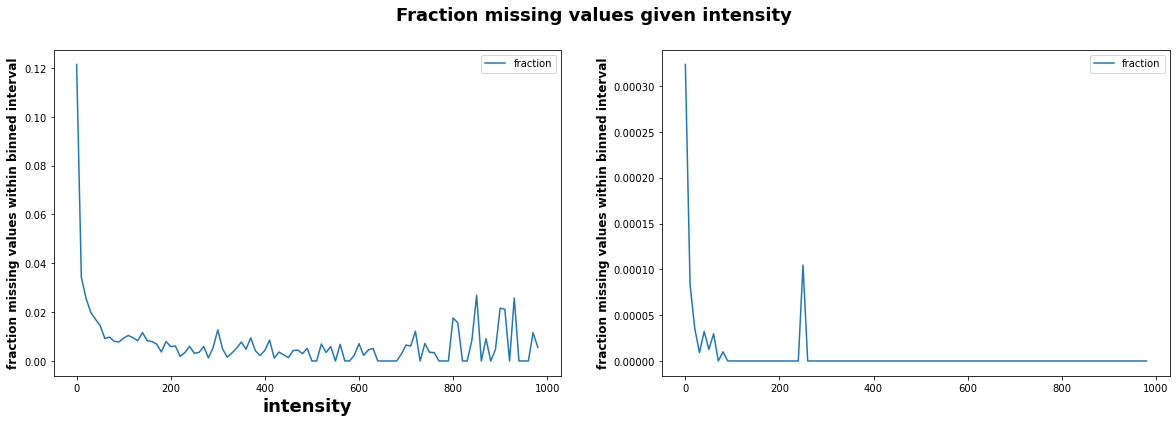
\includegraphics[width=16cm]{../../result/2021-08-13_docs_plots/missingness_fraction_intensity.png}
    \caption{Missingness proportions by observed mean for peptides.}
    \label{fig:missingness_fraction}
\end{figure}


Similarily to DDA data \cite{karpievitch2009statistical} \cite{koopmans2014empirical}, \ref{fig:missingness_fraction} shows that the missing value proportion in DIA data has higher missingness at lower end intensities.  

%* missing values [ok]
%* missing value model [in progress]
%* previous missing value models []
%* censored data [ok]
%* benefit of triqler for missing values [ok]
%* write that the missing value signature is similar for DIA and DDA - compare to A statistical framework for protein quantitation in bottom-up MS-based proteomics fig. 2.
%* missing not at random (Accounting for the Multiple Natures of Missing Values in Label-Free Quantitative Proteomics Data Sets to Compare Imputation Strategies  [18] .) 

% CONT HERE writing about what fig shows and comparing it to [13] figure and writing about misssing not at random model.

\subsection*{DIA methods}
Write about why different methods where used.

\subsubsection*{OpenSwath Analysis}
Version (version) of OpenSwath was used. The spectral library generated above is converted to .pqp format using TargetedFileConverter. Data analysis was conducted using OpenSwathWorkflow with parameters (-Scoring:TransitionGroupPicker:background\_subtraction original -Scoring:stop\_report\_after\_feature -1, -min\_upper\_edge\_dist 1, -tr\_irt hroest\_DIA\_iRT.TraML, -extra\_rt\_extraction\_window 100, -min\_rsq 0.95, -min\_coverage 0.6, -Scoring:Scores:use\_dia\_scores true, -rt\_extraction\_window 600, -mz\_extraction\_window 30, -threads 10, -Scoring:DIAScoring:dia\_extraction\_unit ppm). After data extraction the data .osw output was merged using pyprophet merge option and pyprophet was used for statistical validation. Pyprophet export was used without FDR filtering (--max\_global\_protein\_qvalue 1.0, --max\_global\_peptide\_qvalue 1.0, --max\_rs\_peakgroup\_qvalue 1.0, --max\_transition\_pep 1.0) to give a complete list of peptide quantifications for further down-stream analysis.

\subsubsection*{DIAUmpire and DIA-NN analysis}
DIAUmpire signal extraction (SE) was used through Fragpipe GUI (v15.0). Default parameters was set (MS1 PPM: 10, MS2 PPM: 20, Max Missed Scans:1, Mass Defect Filter On, RP max: 25, RF max: 500, Corr Treshold:0, Delta Apex: 0.2, RT Overlap 0.3, Mass Defect Offset 0.1, Isotope Pattern: 0.3, MS1 SN: 1.1, MS2 SN 1.1, Adjust fragment intensity On). MSFragger was used on the resulting .mzML files from DIAUmpire SE with default parameters for Peak Matching (PPM: [-20, 20], Fragment mass tolerance PPM: 20, Calibration and Optimization: Mass Calibration, Parameter optimization, Isotop error: 0/1, Data type: DDA, ), protein digestion (Load rules: stricttrypsin, Enzyme name: stricttrypsin, Cut after: KR, Cleavage: ENZYMATIC, Missed cleavages: 2, Clip N-term M: On, Peptide length 7-50, Peptide mass range: 500-5000, Split database: 1) and Modification (Variable modifications: M, \/[\^, Fixed modification: "all selected"). 

\subsubsection*{EncyclopeDIA and PECAN analysis}
Prosit was used to construct spectra libraries from the modified FASTA files. The fragmentation model used was "Prosit - Model - Fragmentation" and the iRT model "Prosit - Model - iRT" (available from \url{https://figshare.com/projects/Prosit/35582)}.
...

\subsection*{Protein quantification methods}

\subsubsection*{Triqler}

Triqler is based on probabilistic graphical models that allow error information to propagate through all steps from MS1 feature detection to protein quantification. Unconventionally, it produces posterior probabilities for fold changes rather than point estimates \cite{The2018Integrated}. The robustness of results when faulty imputation of missing data is conducted is a common problem in missing data analysis \cite{ma2018bayesian} and imputation methods for missing values can introduce various type of errors, which can have significant impact on differential abundances \cite{webb2015review} \cite{lazar2016accounting}. These posteriors incorporate information about uncertainty at different levels of the protein quantification process, and therefore should result in robust protein quantification. Specifically, It combines combines the identification and quantification errors from feature, PSM, peptide, protein and treatment group level to a final posterior distribution of fold change between two treatment groups. Triqler has been shown to distinguish more proteins for DDA data compared to other DDA protein quantification methods. \cite{The2018Integrated}. 

Triqler was used with --fold\_change\_eval between 0-2 with 0.04 increments. It computes the two-sided differential probability threshold between the two samples given a fold change evaluation limit. 

\subsubsection*{Top3}
The precursors are filtered by q-value \textgreater 1\% and the average of the three largest peptide intensities are taken for each protein. Protein with only one detected peptide (single hit proteins) and proteins detected only in two injections are discarded.

\subsubsection*{MSstat}
 MSstats customizes a linear mixed model to the specific experiment and each protein \cite{choi2014msstats}. SWATH2Stats was used to convert the .osw output files to MSStats input format. dataProcess function in the MSstats package is used for data pre-processing and quality control of the MS runs of the data into quantitative data for model fitting and group comparison (Default parameters was used (specifically the peptide-level data is filtered by an m-score < 0.01 to reduce the memory consumption before running MSstats). quantification function in the MSstats package is applied on the pre-processed data to generate the quantification results for each protein.  

\subsubsection*{Msqrobsum}
Msqrobsum provides protein summarization that account for peptide specific effect (MSqRob inference framework \cite{goeminne2020msqrob}) and are further processed using robust ridge regression. The MSqRob inference frame work is a linea regression peptide-based mixed model. The parameters for the model are tuned using penalised estimation and multiple-testing is corrected using Benjamini-Hochberg FDR procedure. 

The data is processed according to default setting. It preprocessed using MSnBase R/Bioconductor package \cite{gatto2012msnbase} and normalized using Variance Stabilizing Normalization \cite{von2002variance}. 


%(Note: write something about difference FDR computation method and conservativeness, and why it does not make sense to compare between processing method, but it is ok to compare between post-processing methods)



\subsection*{Benchmarking methods}

\subsubsection*{Variance Structure - why the DDA methods works and makes sense}
The field of protein quantification is relatively new. Many protein quantification methods have been developed for LFQ data and performance has been established on DDA data. Many of these methods should be generalizable for DIA data. Triqler (probabilistic graphical model), MsStats (linear mixed model) and MSqRob (Ridge Regression) all require a homoskedastic variance. This is investigated using statistical visualization of the data.

\subsubsection*{Protein level results}

\subsubsection*{Differential abundance - log2distribution and number of differentially abundant proteins}
The differentially abundant proteins are proteins with a log2-fold change of proteins with a q-value lower than a certain threshold for q-value based protein summarization methods (Top3, msStats and msqrob), while triqler computes a posterior distribution based  log2-fold change. 

%(Write formula for triqler)
%(Write formula for other methods)

\subsubsection*{FDR control (calibration plot)}
An FDR control of the quanfication method is used to check the calibration of the methods. We check the true FDR against the reported FDR. The true FDR is estimated using

\[ \text{True} \: FDR = \frac{FP_\text{estimate, specie}}{DE \:\text{Proteins}_\text{specie}}\]

for each E.coli and yeast. The human protein are used to compute the $FP_\text{estimate}$ for each specie. We assume the proportion human proteins that are differentially abundant at a given FDR-level is the proportion $FP$ for E.Coli and yeast as well, this proportion is denoted as a constant scaling factor $k$. The $F_\text{estimate}$ is therefore

\[ FP_\text{estimate, specie} = k \cdot \text{Protein}_\text{specie} \]

where

\[ k = \frac{DE \: \text{Protein}_\text{human}}{\text{Protein}_\text{human}}\]



%An FDR control of the quantification methods is required for benchmarking. We use the False Discovery Proportion (FDP) and True Positive Rate (TPR). FDP is calculated using and calculated using 

%	\[FDP = \frac{ \text{false positives}}{\text{true positive} + \text{false positive}} \]

%and,

%	\[TPR = \frac{\text{true positives}}{\text{all positives}} \]


%The FDP is calculated using the fraction of human proteins discovered as DE and the TP is the fraction of E.Coli and Yeast discovered. 

\end{comment}


\section*{Results}


\begin{table}[H]
\begin{tabular}{lllllll}
\hline
\multicolumn{7}{c}{OSW}                                                                                                                                                                                   \\ \hline
Condition & \multicolumn{3}{c}{1}                                                                         & \multicolumn{3}{c}{2}                                                                         \\
Run       & \multicolumn{1}{c}{002-Pedro} & \multicolumn{1}{c}{004-Pedro} & \multicolumn{1}{c}{006-Pedro} & \multicolumn{1}{c}{003-Pedro} & \multicolumn{1}{c}{005-Pedro} & \multicolumn{1}{c}{007-Pedro} \\
Peptides  & 20 747                        & 21 445                        & 21 016                        & 20 494                        & 22 792                        & 22 787                        \\
Proteins  & 2 836                         & 2 857                         & 2 869                         & 2 818                         & 2 909                         & 2 918                         \\ \hline
\end{tabular}
 \caption{{\bf Number of identified peptides and proteins for the samples using OSW.}
      \label{fig:osw_peptide_and_protein_id}}
\end{table}

\begin{table}[H]
\begin{tabular}{lllllll}
\hline
\multicolumn{7}{c}{DIANN}                                                                                                                                                                                 \\ \hline
Condition & \multicolumn{3}{c}{1}                                                                         & \multicolumn{3}{c}{2}                                                                         \\
Run       & \multicolumn{1}{c}{002-Pedro} & \multicolumn{1}{c}{004-Pedro} & \multicolumn{1}{c}{006-Pedro} & \multicolumn{1}{c}{003-Pedro} & \multicolumn{1}{c}{005-Pedro} & \multicolumn{1}{c}{007-Pedro} \\
Peptides  & 21 036                        & 20 783                        & 21 040                        & 21 243                        & 21 325                        & 21 248                        \\
Proteins  & 3 377                         & 3 350                         & 3 368                         & 3 358                         & 3 381                         & 3 356                         \\ \hline
\end{tabular}
 \caption{{\bf Number of identified peptides and proteins for the samples using DIANN.}
      \label{fig:diann_peptide_and_protein_id}}
\end{table}

\subsection*{Test of assumptions}

We strived to validate the Triqler method for a DIA setting. We hence investigatred some properties of DIA data to see if they agree with the assumption we mnade when designing Triqler for DDA data. DIA data is known to encompass a larger dynamic range than DDA data \citation{FIXME}. This could affect one of Triqles assumptions, that the noise structure is mainly multiplicative, i.e. that the standard deviation within a sample group is proportional to its mean. When investigating all the peptide abundance measurements at a 1\% identification FDR from the TripleTOF6600 section of the LFQBench dataset, we found a relatively linear relation between standard deviation and mean (Figure \ref{fig:assumptions}A). Further, Triqler assumes that the missing peptide abundance values follow a xxx distribution, which is also roughly fullfilled by DIA data (See Figure \ref{fig:assumptions}B).


\begin{figure}[htb]
    \centering
    \begin{tabular}{lc} 
    A & 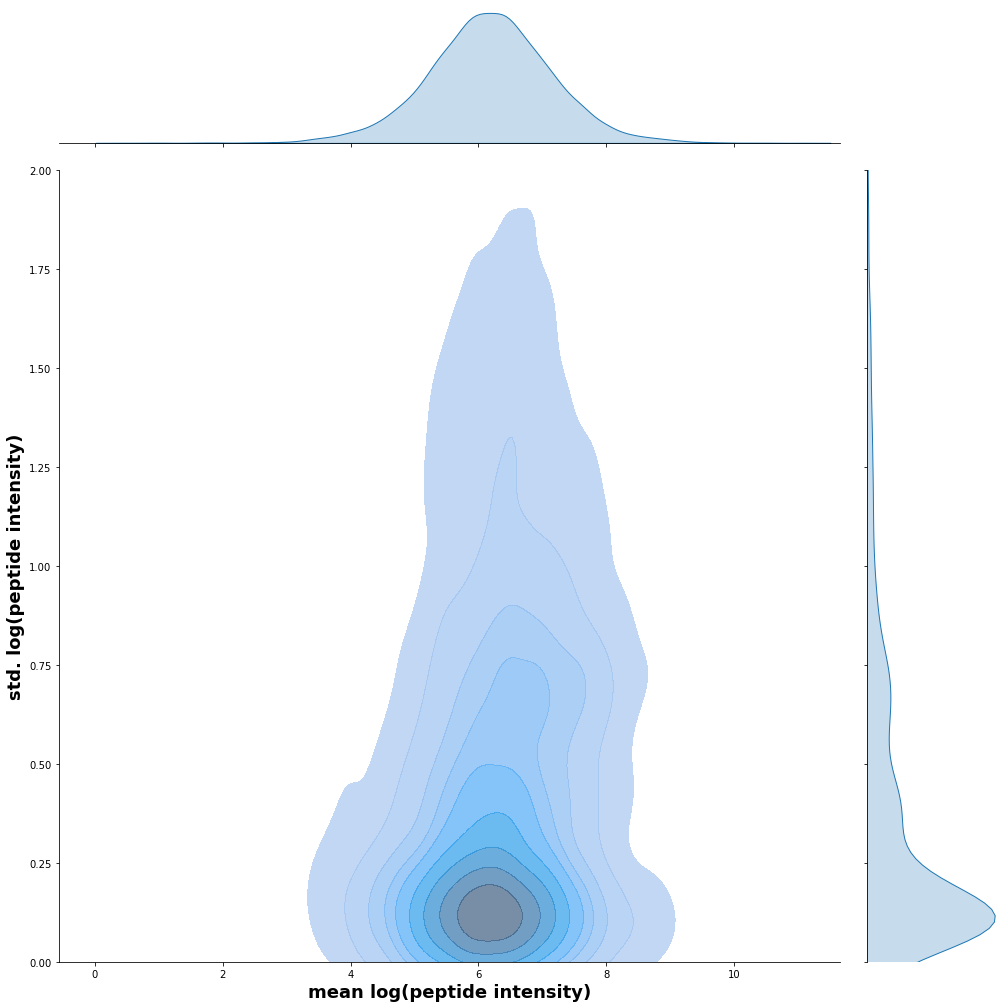
\includegraphics[width=0.6\linewidth]{../../result/report_plots/peptide_mu_vs_std.png} \\
    B & %\includegraphics[width=0.3\linewidth]{FIXME}
    \end{tabular}
    \caption{{\bf (THIS IS OLD THE PLOT)The assumtions that Triqler makes about peptide abundance values are valid also for DIA data in the TripleTOF6600 section of the LFQ Bench set.}  (A) We plotted the standard deviation as a function of the mean of every peptide  in log-log scale. We observe a nearly uniform offset in standard deviation across the intensity scale, demonstrating that $\log(\sigma) \approx \log(\mu) + \log(k)$ and hence   $\sigma \approx \mu k$ (B) We plotted the fraction of peptides observing one missing value for each triplicate in the set. We obseve that this empirical distribution roughly follows the assumed function FIXME.}
      \label{fig:assumptions}
\end{figure}



\begin{figure}[H]
    \centering
    \begin{tabular}{lclc} 
        A 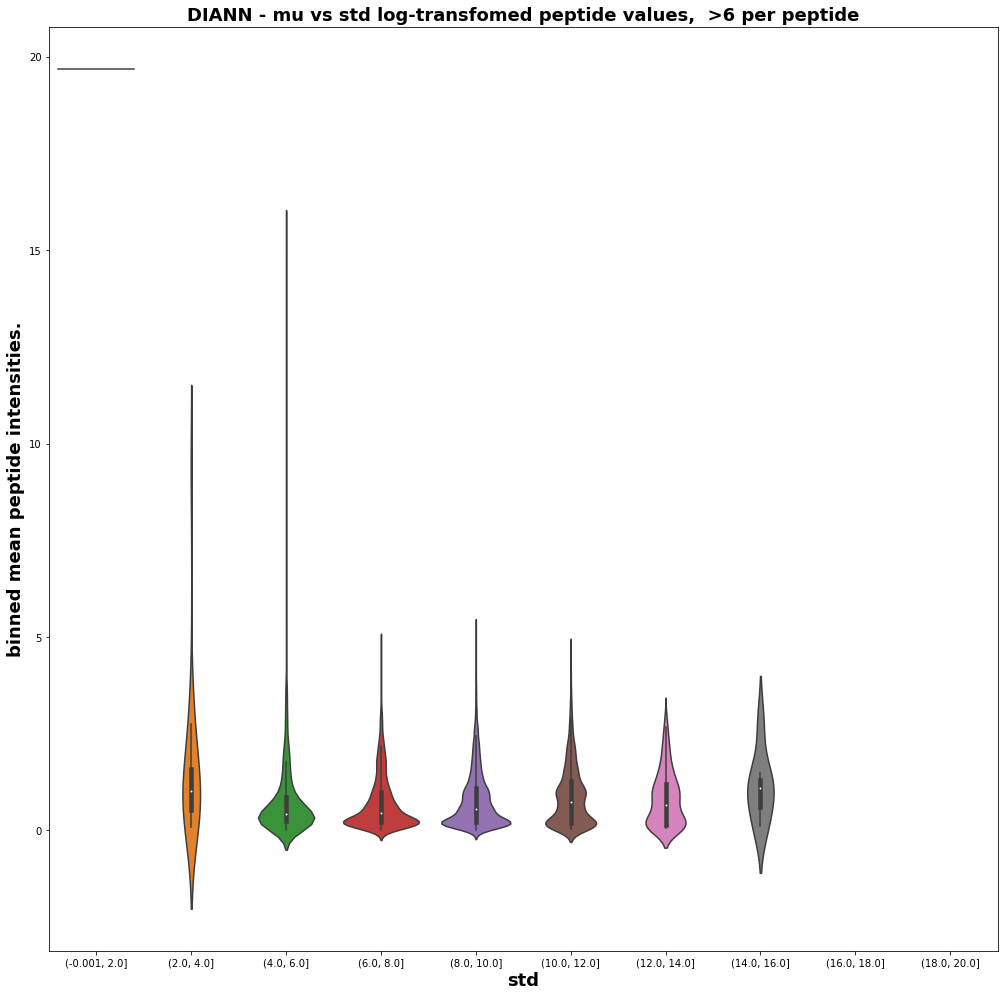
\includegraphics[width=0.5\linewidth]{../../result/report_plots/osw_sigma_mu_violinplot_filtered.png}  & &%\includegraphics[width=0.3\linewidth]{} & 
        C 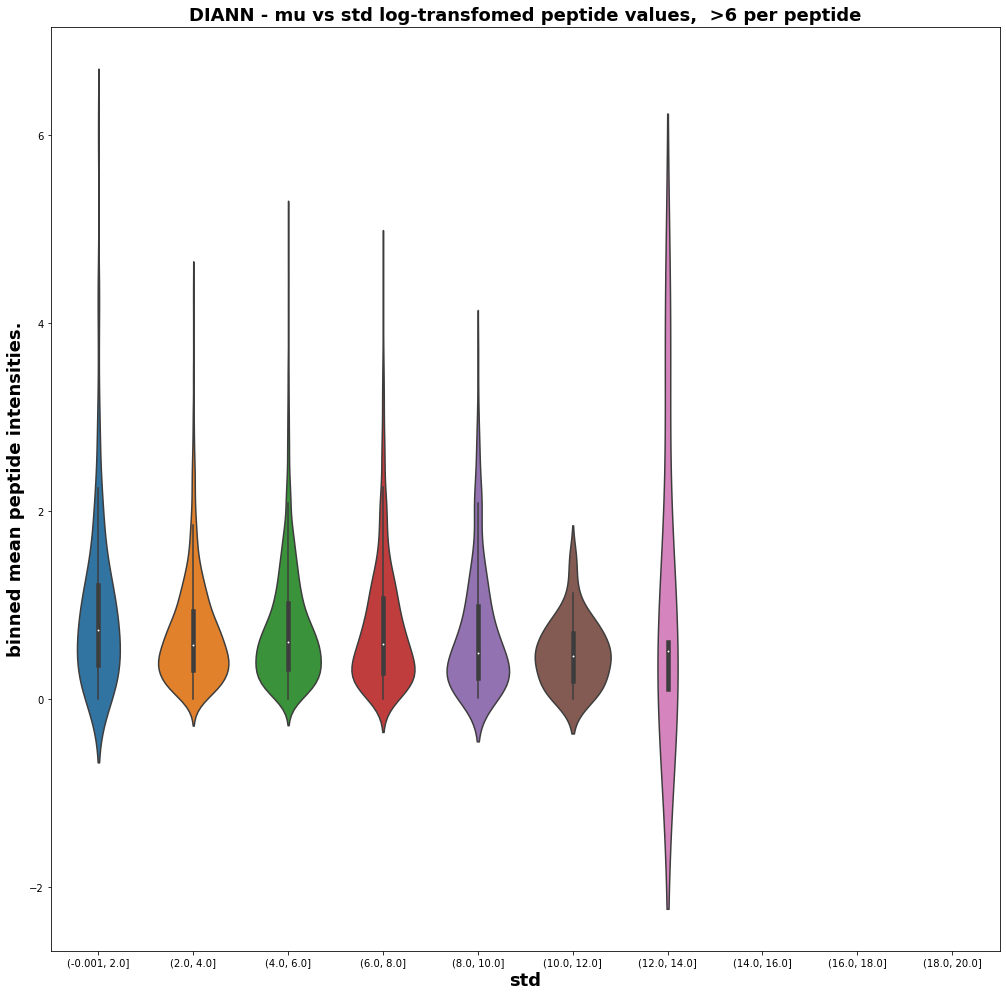
\includegraphics[width=0.5\linewidth]{../../result/report_plots/diann_sigma_mu_violinplot_filtered.png} & \\%\includegraphics[width=0.3\linewidth]{} \\ 
    \end{tabular}
    \caption{{\bf The assumtions that Triqler makes about peptide abundance values are valid also for DIA data in the TripleTOF6600 section of the LFQ Bench set.}  (A) We plotted the standard deviation as a function of the mean of every peptide  in log-log scale. We observe a nearly uniform offset in standard deviation across the intensity scale, demonstrating that $\log(\sigma) \approx \log(\mu) + \log(k)$ and hence   $\sigma \approx \mu k$ (B) We plotted the fraction of peptides observing one missing value for each triplicate in the set. We obseve that this empirical distribution roughly follows the assumed function FIXME.}
      \label{fig:assumptions}
\end{figure}



\subsection*{Test of performance}

We wanted to compare the performance of Triqler against other protein summarization methods. An inherent problem when comparing different protein summarization softwares is that the performance is affected by which protein inference structure is used, in a data set dependent manner \cite{serang2012recognizing}. For example, when reporting number of differentially abundant proteins in protein mixtures, a protein inference scheme that infer any protein contain  a detected peptide will report more differentially abundant proteins than more restrictive scheme that just report a parsimonous set of proteins when benchmarking with mixtures of cell lysate mixtures data sets. \todo{find the prefered term for ``cell lysate mixture''} For such data sets there is no mechanisms restrictive mechanism detecting situations where non-present proteoforms are reported as long as they are part of and reported with protein abundance rates compatible to the right proteome. To elaviate, or at least minimize, this problem from our comparison, we restricted the searched FASTA files by removing proteins with shared peptides. This should give a fair comparison of protein summarization regardless of the protein inference method.

Also, we selected to compare the efficency of Triqler to the ones of the protein summarization strategies from msStats, msSqRobSum and Top-3 using two different processing strategies, spectral libraries using DDA data, and when generating pseudo-spectra with DIA-Umpire~\cite{tsou2015dia}. Here we selected to run Triqler with a lower bound estimate as described in The\&K\"{a}ll~\cite{the2021triqler}, which ended up as FIXME for the spectral library data, and FIXME for the psudo-spectra enabled data.

\subsubsection*{Fold change distributions}

To get an overview of the results of the methods we first made histograms of the reported protein level fold-changes as reported by the compared methods in Figure \ref{fig:fc_histogram}.  

\begin{figure}[hbt]
    \centering
    %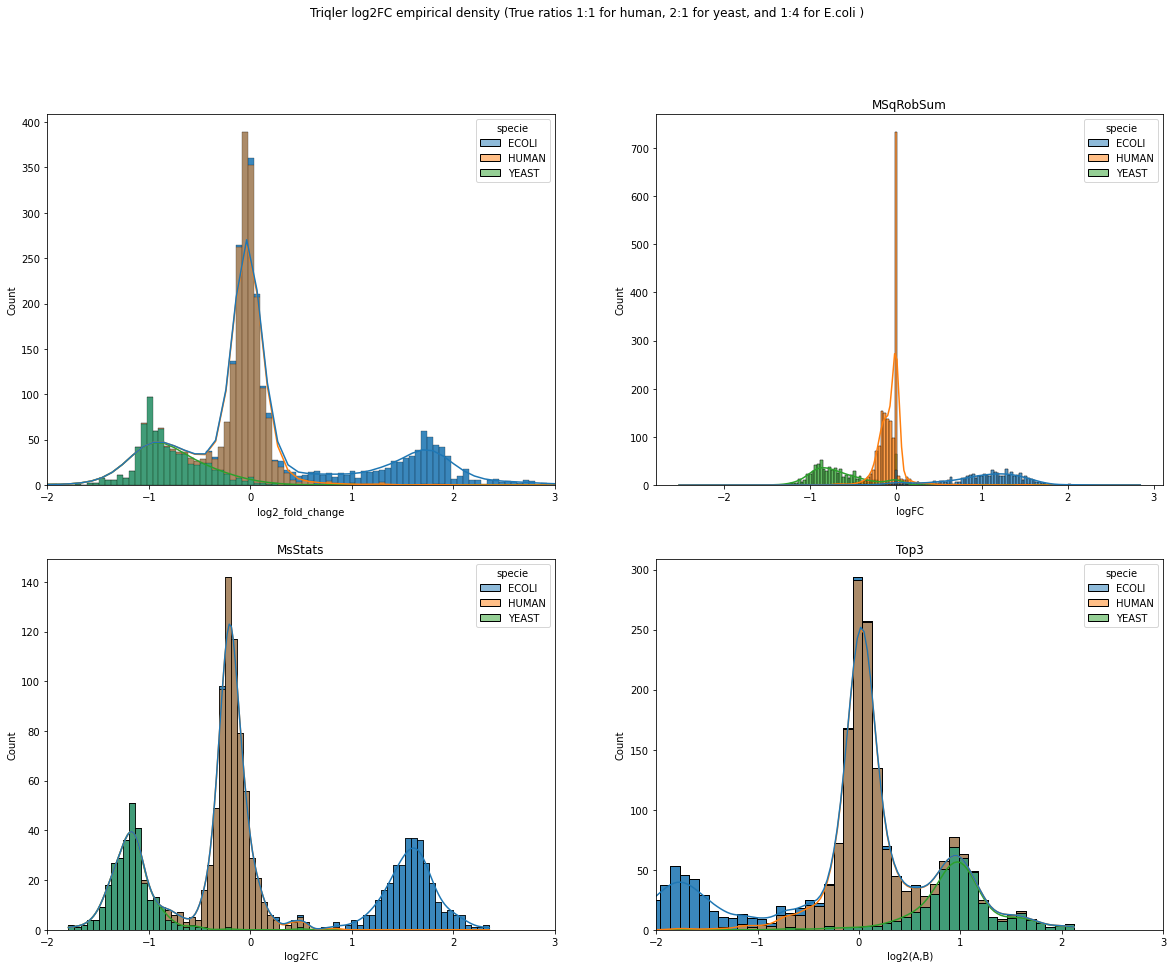
\includegraphics[width=16cm]{../../result/2021-08-13_docs_plots/intensity_plot.png}
    \begin{tabular}{lclc} 
        A 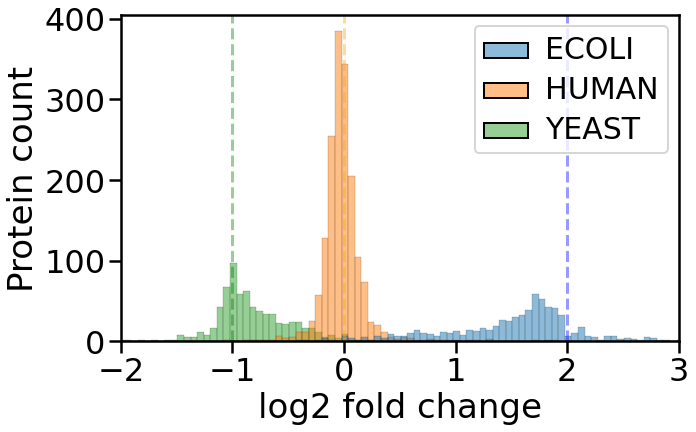
\includegraphics[width=0.4\linewidth]{../../result/report_plots/osw_triqler_intensity.png} & &%\includegraphics[width=0.3\linewidth]{} & 
        E 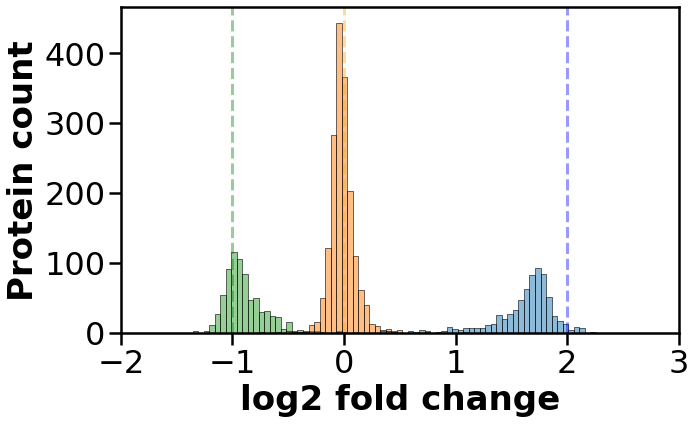
\includegraphics[width=0.4\linewidth]{../../result/report_plots/diann_triqler_intensity.png} & \\%\includegraphics[width=0.3\linewidth]{} \\ 
        B 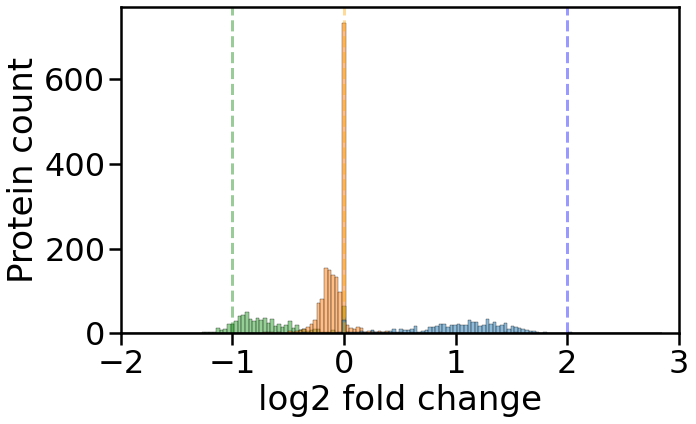
\includegraphics[width=0.4\linewidth]{../../result/report_plots/osw_msqrobsum_intensity.png} & &%\includegraphics[width=0.3\linewidth]{} & 
        F 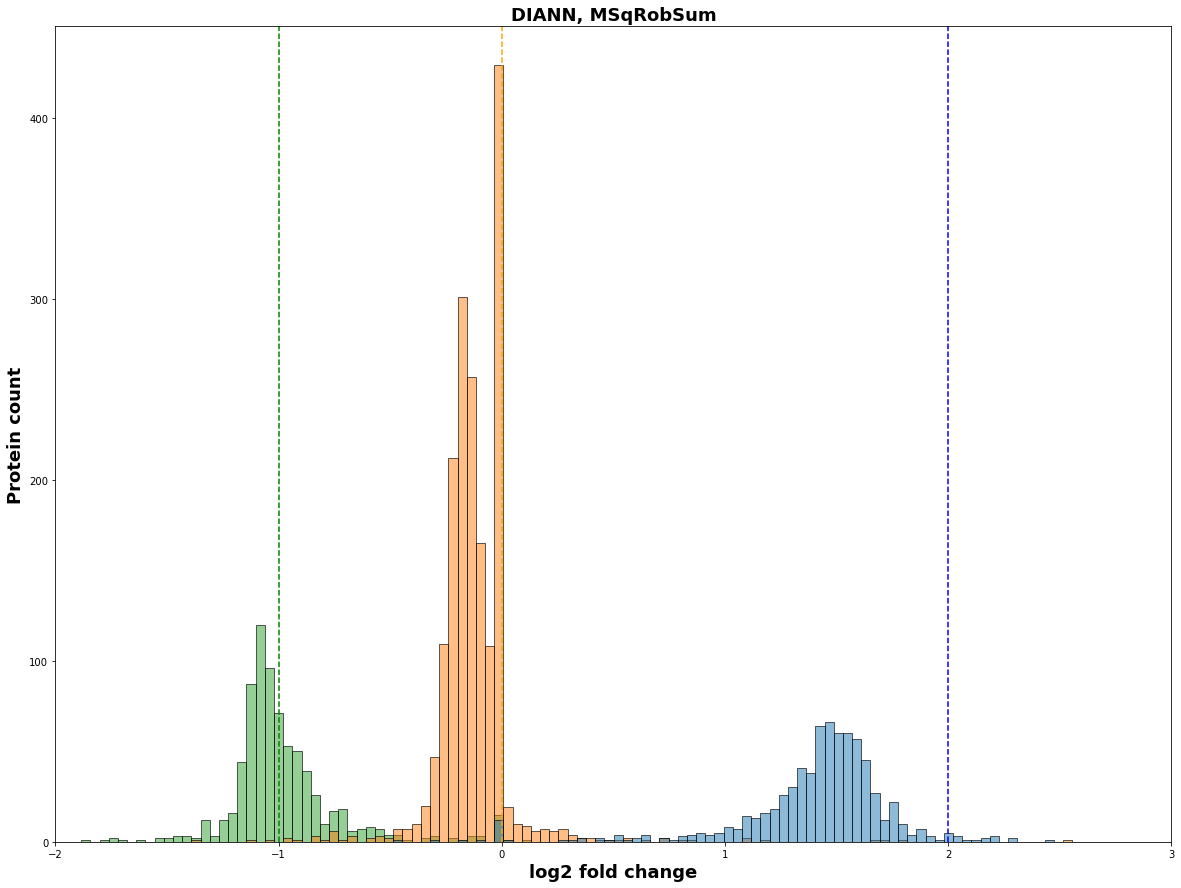
\includegraphics[width=0.4\linewidth]{../../result/report_plots/diann_msqrobsum_intensity.png} & \\%\includegraphics[width=0.3\linewidth]{} \\ 
        C 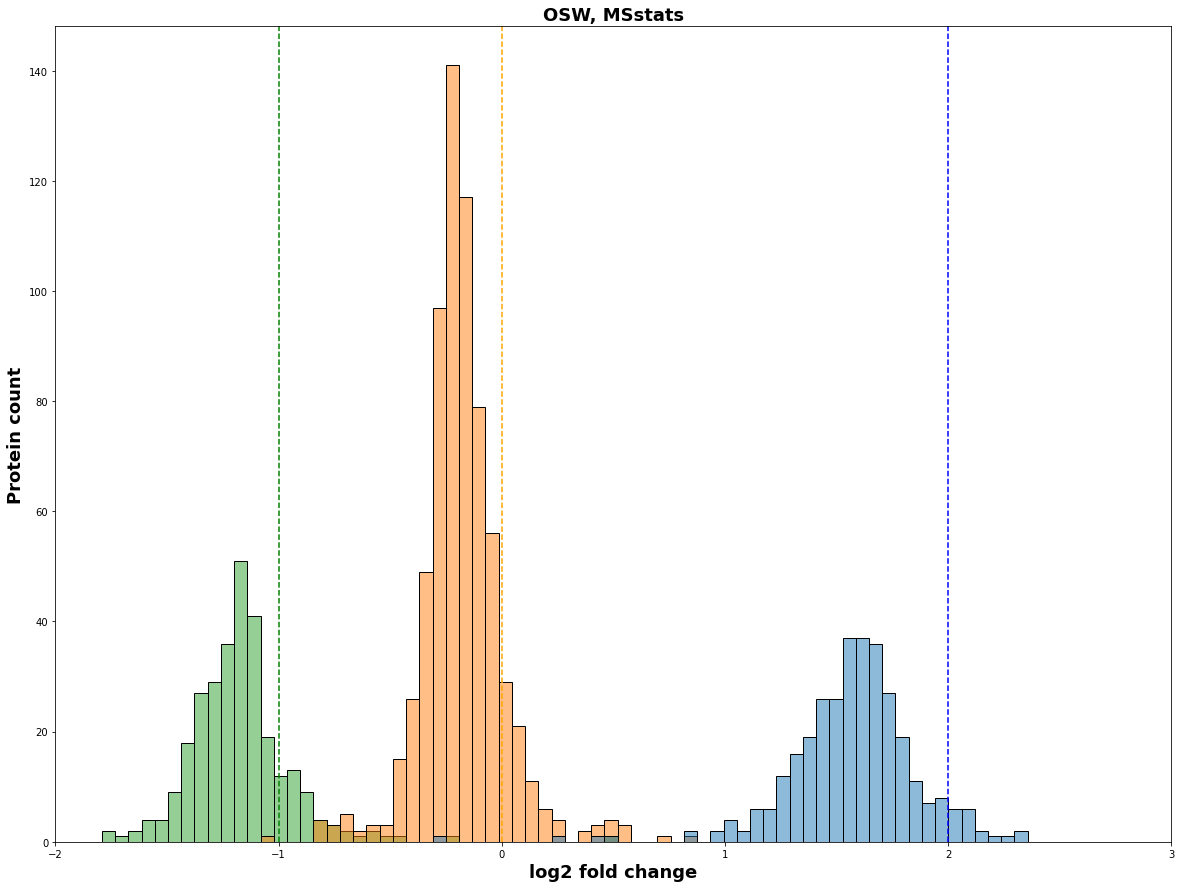
\includegraphics[width=0.4\linewidth]{../../result/report_plots/osw_msstats_intensity.png} & &%\includegraphics[width=0.3\linewidth]{} & 
        G 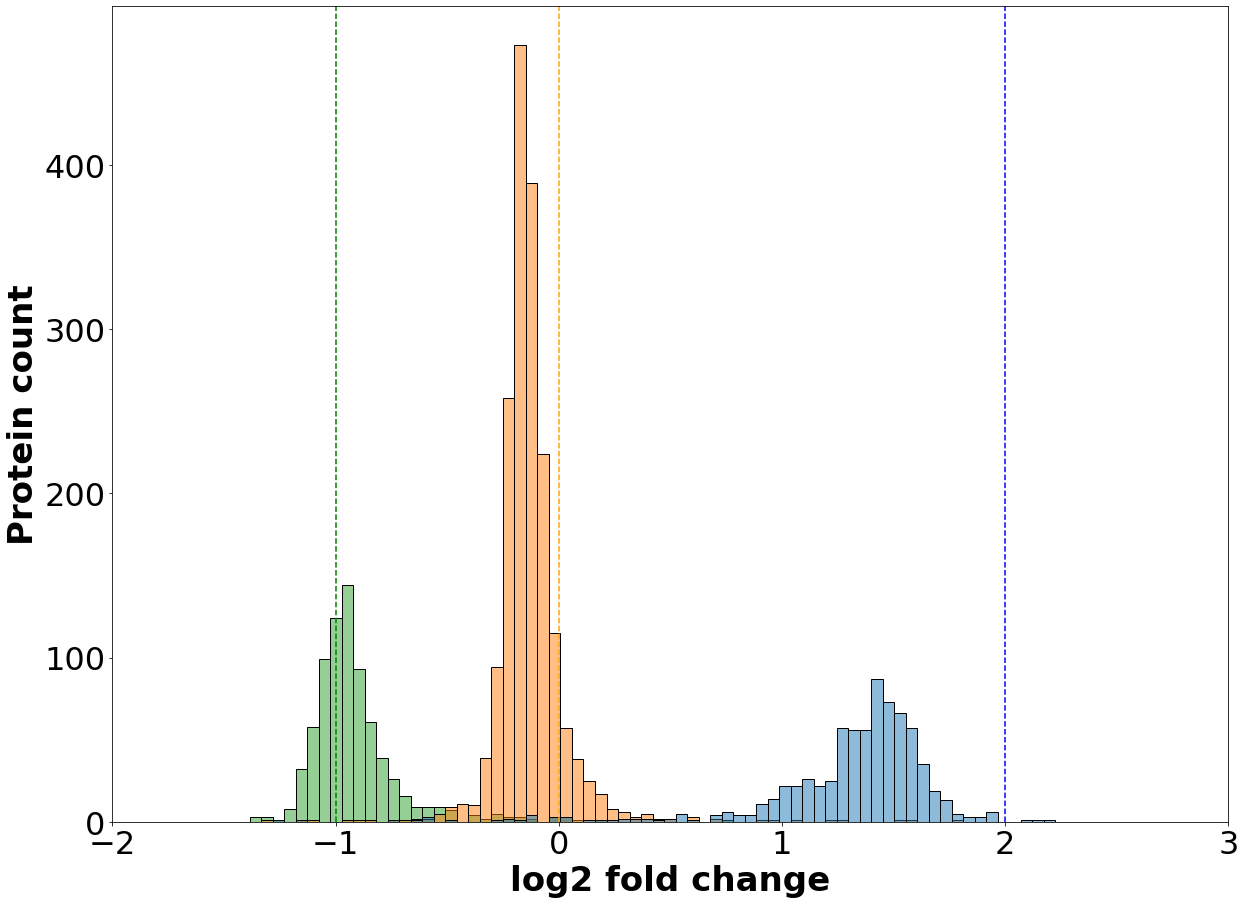
\includegraphics[width=0.4\linewidth]{../../result/report_plots/diann_msstats_intensity.png} & \\%\includegraphics[width=0.3\linewidth]{} \\ 
        D 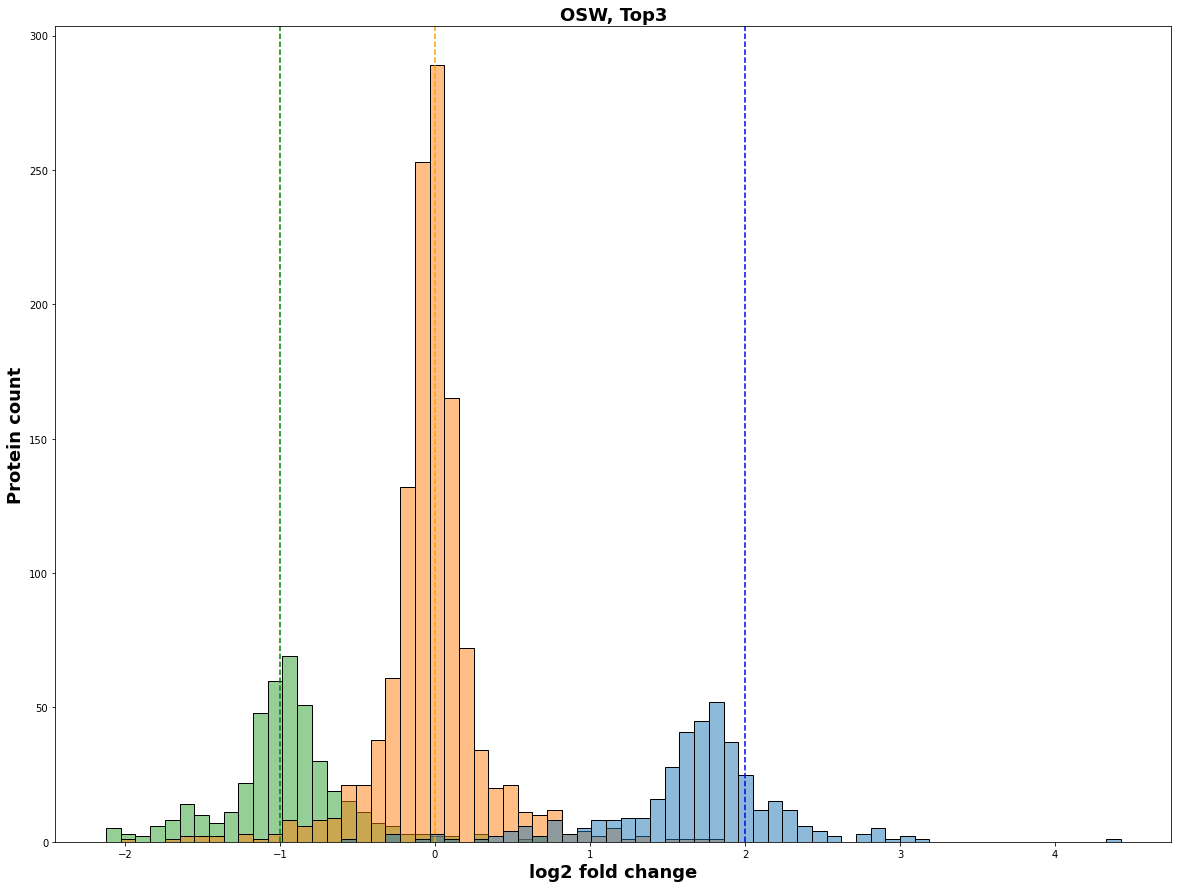
\includegraphics[width=0.4\linewidth]{../../result/report_plots/osw_top3_intensity.png} & &%\includegraphics[width=0.3\linewidth]{} & 
        H 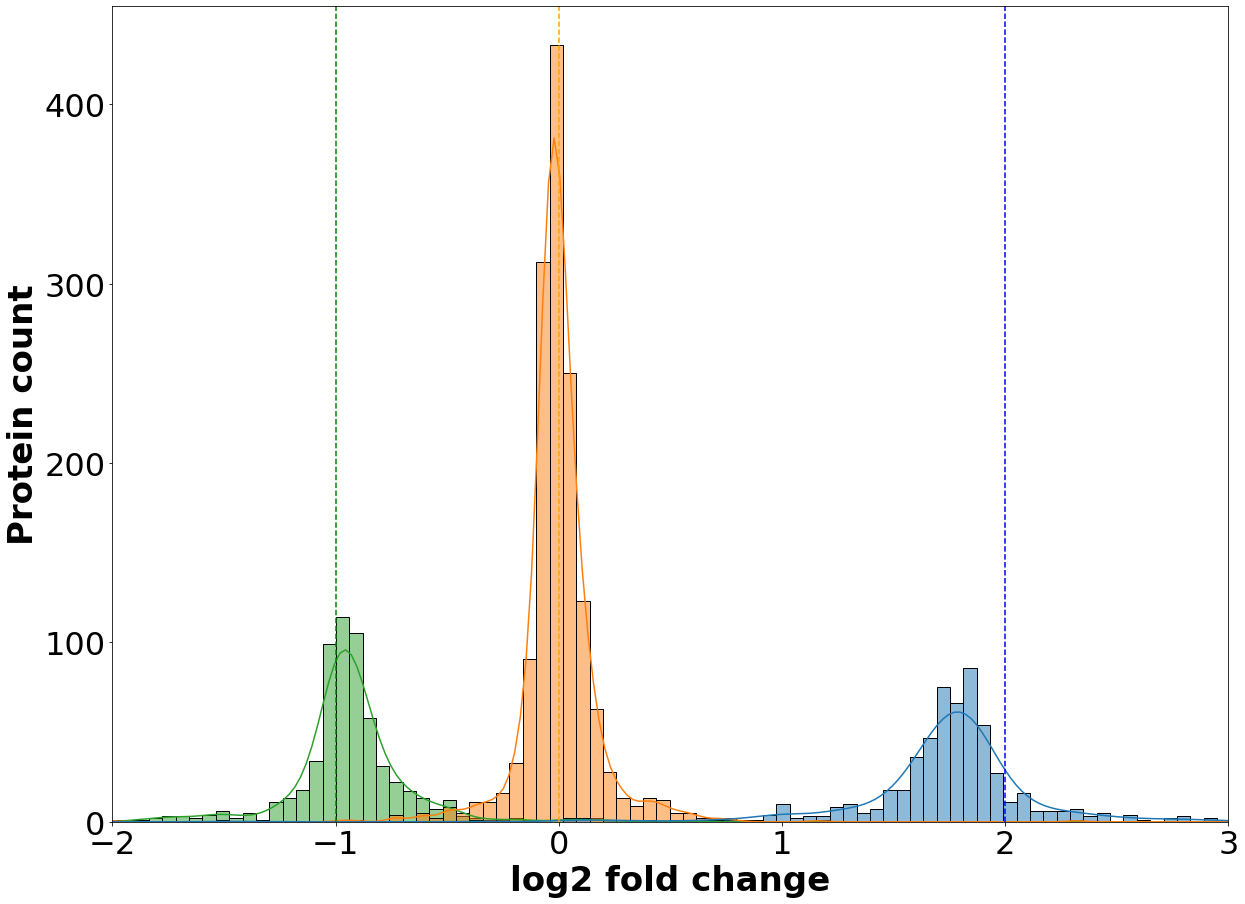
\includegraphics[width=0.4\linewidth]{../../result/report_plots/diann_top3_intensity.png} & %\includegraphics[width=0.3\linewidth]{} 
    \end{tabular}
    \todo[inline]{Make the corresponding histograms, one png per histogram. Alternatively do a sns.PairGrid with shared axes with 8 subpanels and a shared legend.}
    \caption{{\bf Comparison of reported fold change distributions.} We used peptide data from (A-D) DDA spectrum libraries and (E-H) psedo spectra as generated by 
    (A,E) Triqler, (B,F) MSqRobSum, (C,G) MSstats, and (D,H) Top-3. \label{fig:fc_histogram}}
\end{figure}


%        A & &%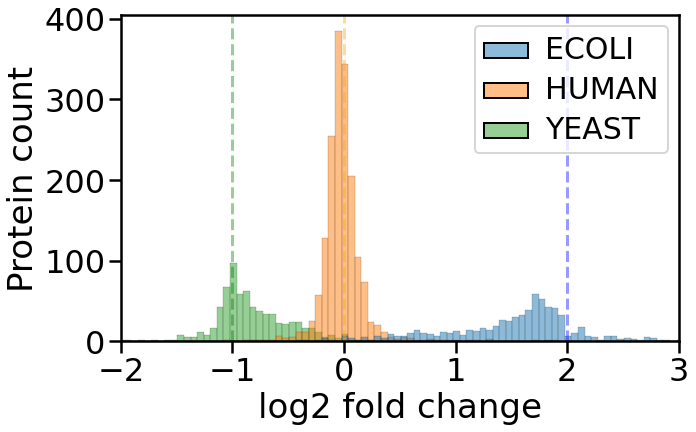
\includegraphics[width=0.3\linewidth]{../../result/report_plots/osw_triqler_intensity.png} & 
%        E & %\\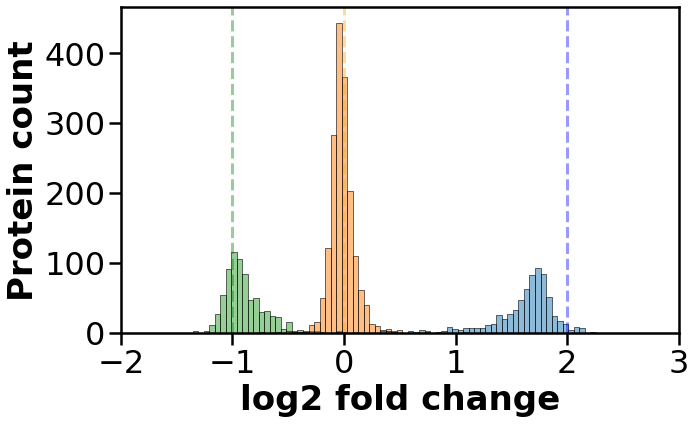
\includegraphics[width=0.3\linewidth]{../../result/report_plots/diann_triqler_intensity.png} \\ 
%        B & &%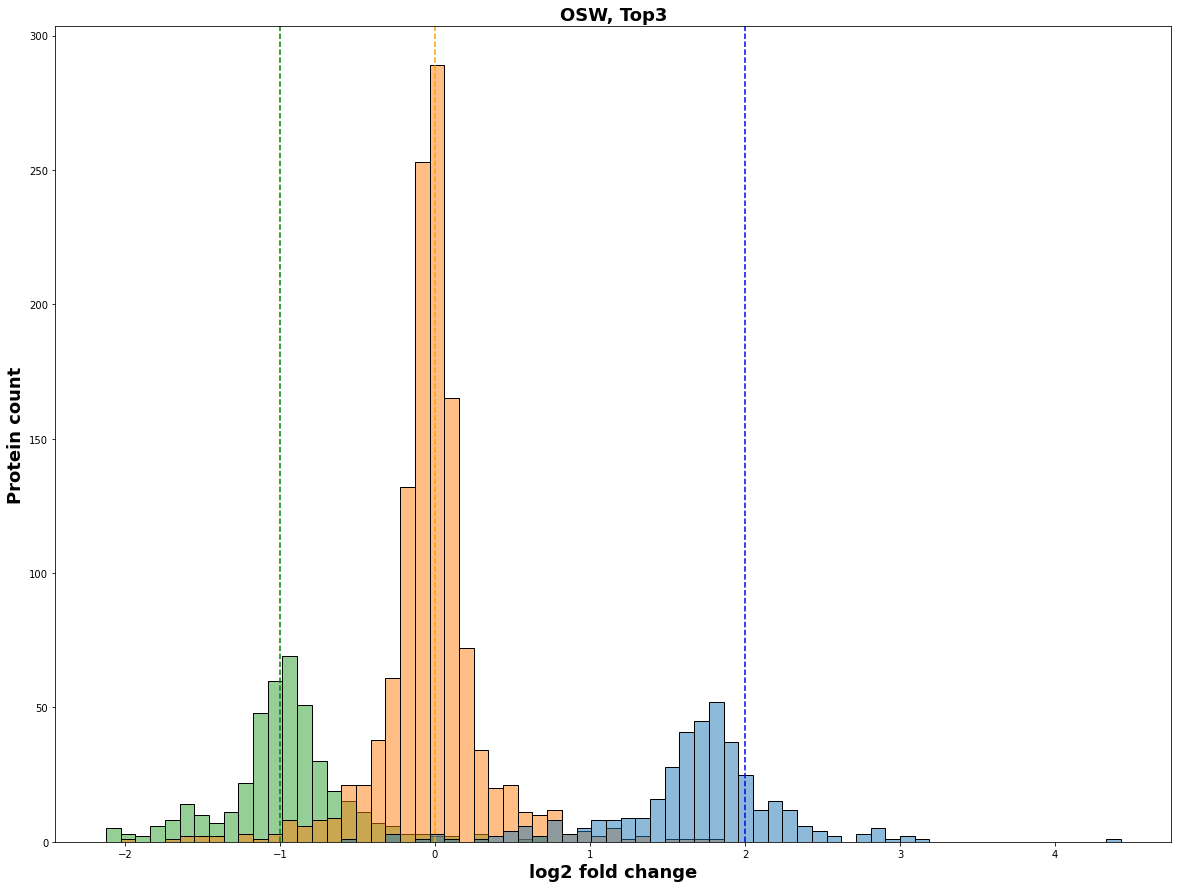
\includegraphics[width=0.3\linewidth]{../../result/report_plots/osw_top3_intensity.png} & 
%        F & %\\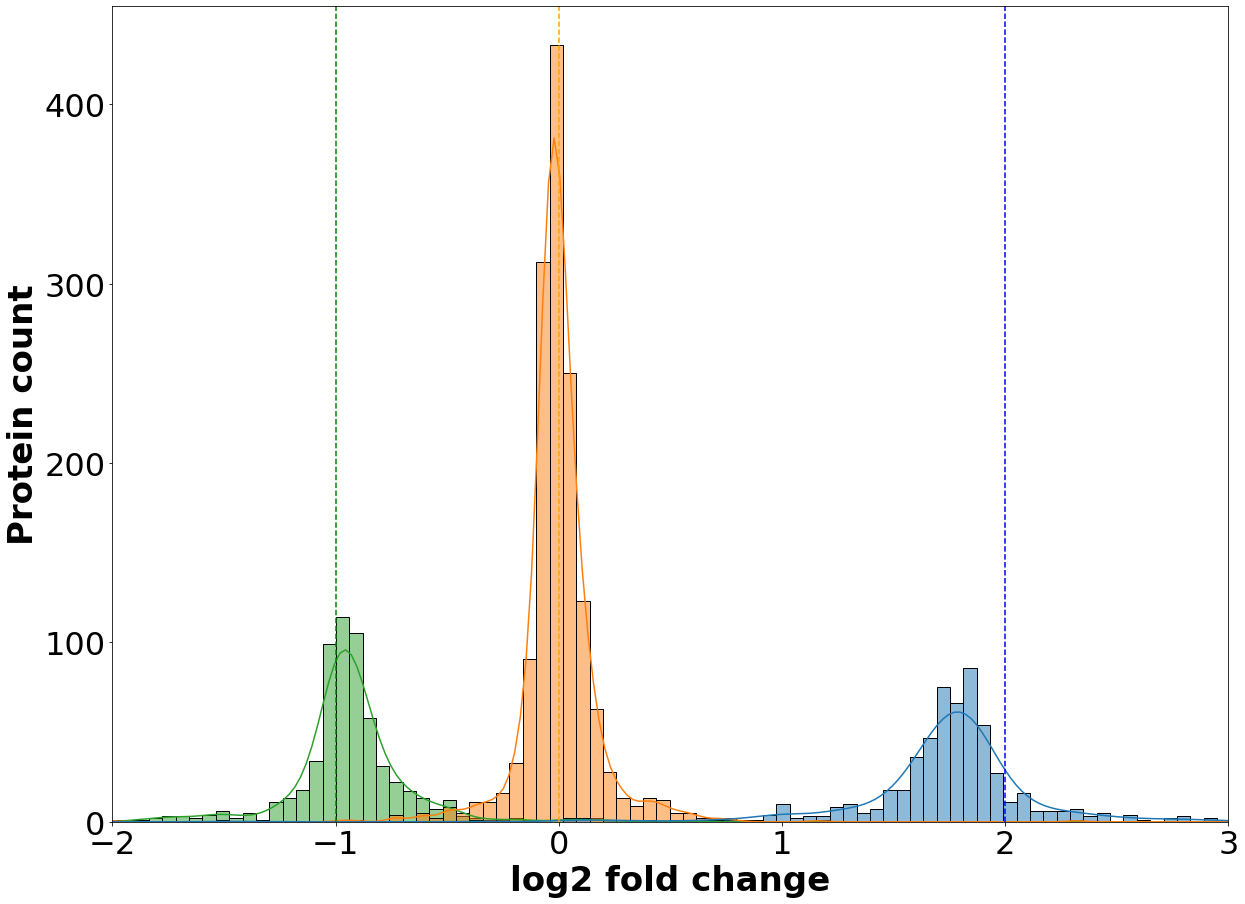
\includegraphics[width=0.3\linewidth]{../../result/report_plots/diann_top3_intensity.png} \\ 
%        C & &%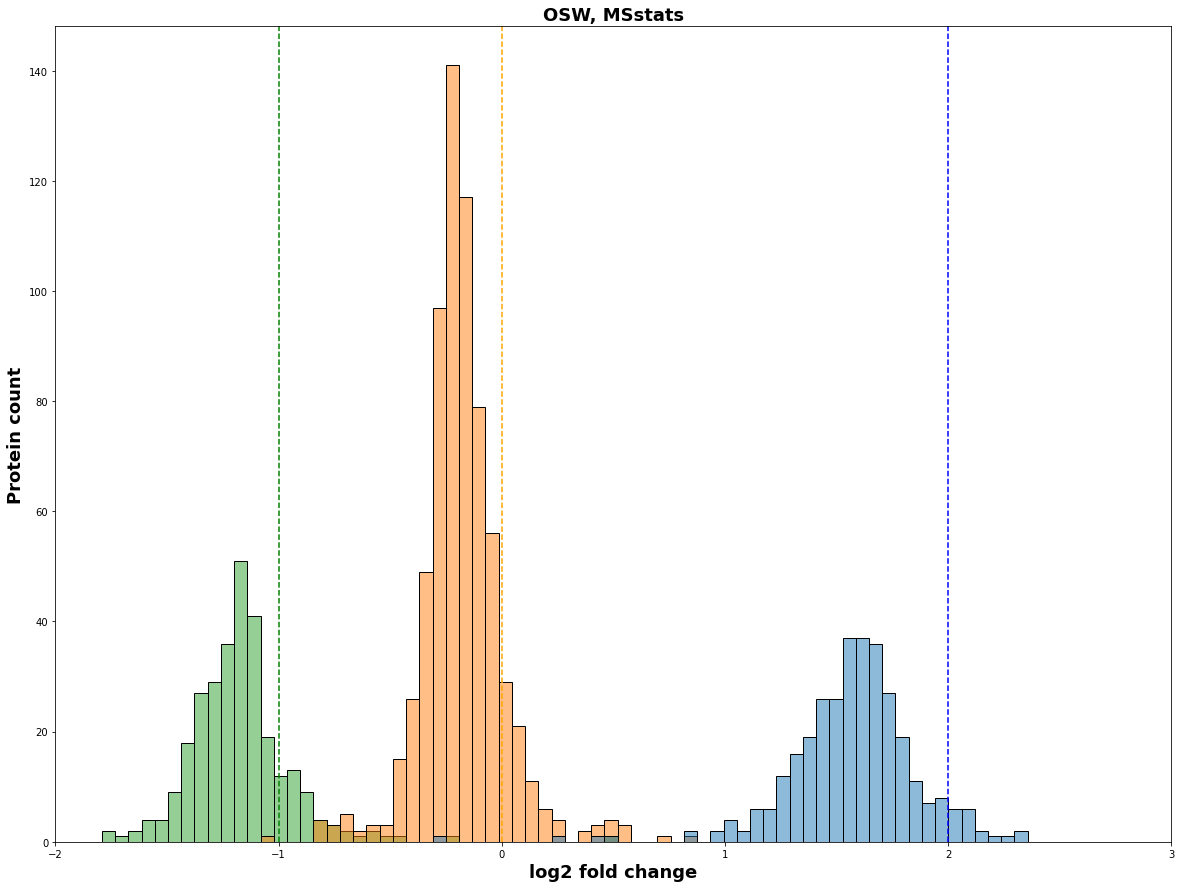
\includegraphics[width=0.3\linewidth]{../../result/report_plots/osw_msstats_intensity.png} & 
%        G & %\\\includegraphics[width=0.3\linewidth]{../../result/report_plots/diann_msstat_intensity.png} \\ 
%        D & &%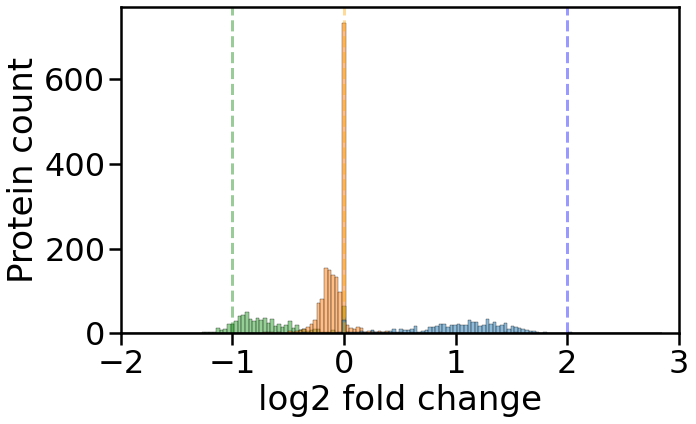
\includegraphics[width=0.3\linewidth]{../../result/report_plots/osw_msqrobsum_intensity.png} & 
%        H & %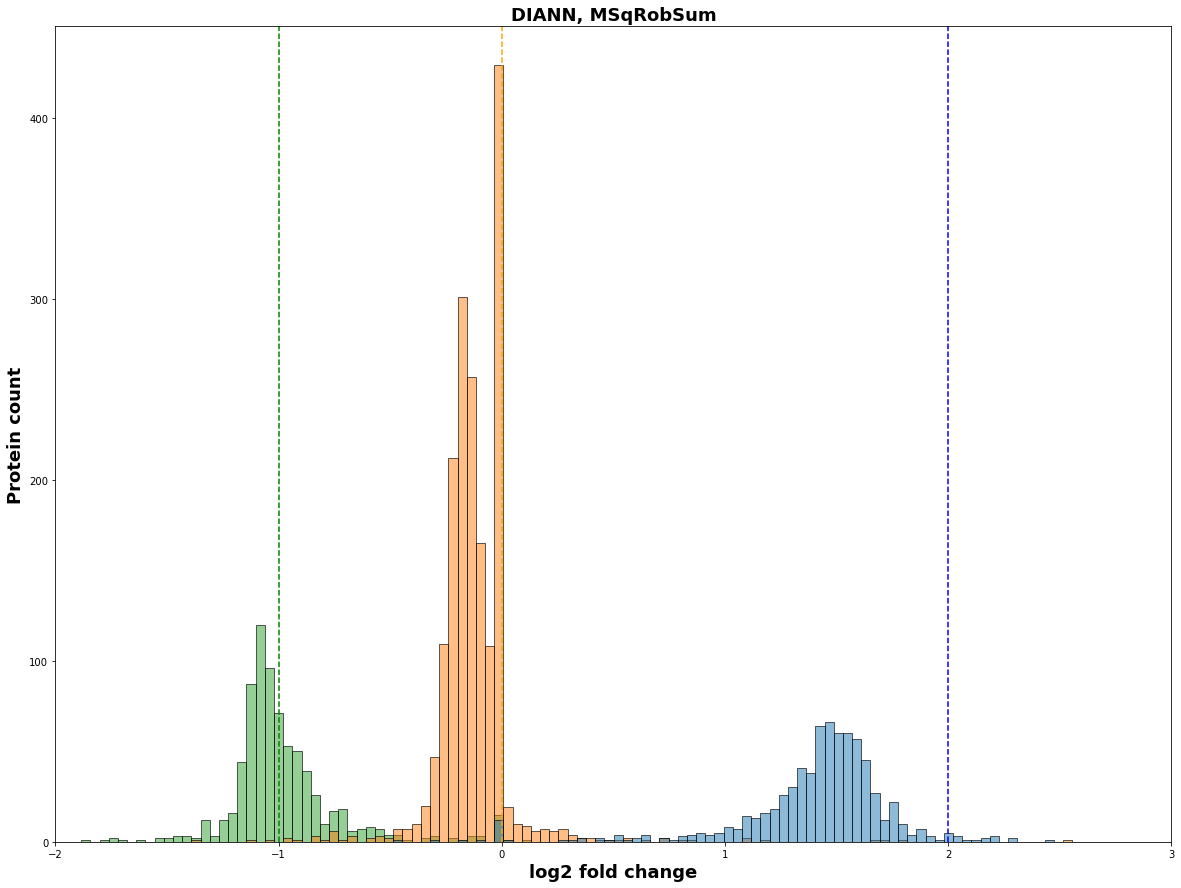
\includegraphics[width=0.3\linewidth]{../../result/report_plots/diann_msqrobsum_intensity.png} 

\subsubsection*{Comparison of ability to differentiate differentially abundant proteins}

The LFQBench set contain varying concentrations of {\em E. Coli} and Yeast concentrations in a background of HeLa-cells. As a first test of performance we compared the methods'ability to inferr differentially abundant {\em E. Coli} and Yeast protein as a function of the number of false positives from the HeLa-background, see Figure \ref{fig:diff_vs_hela}. Overall it seems like 


\begin{figure}[hbt]
    \centering
    \begin{tabular}{lclc} 
        %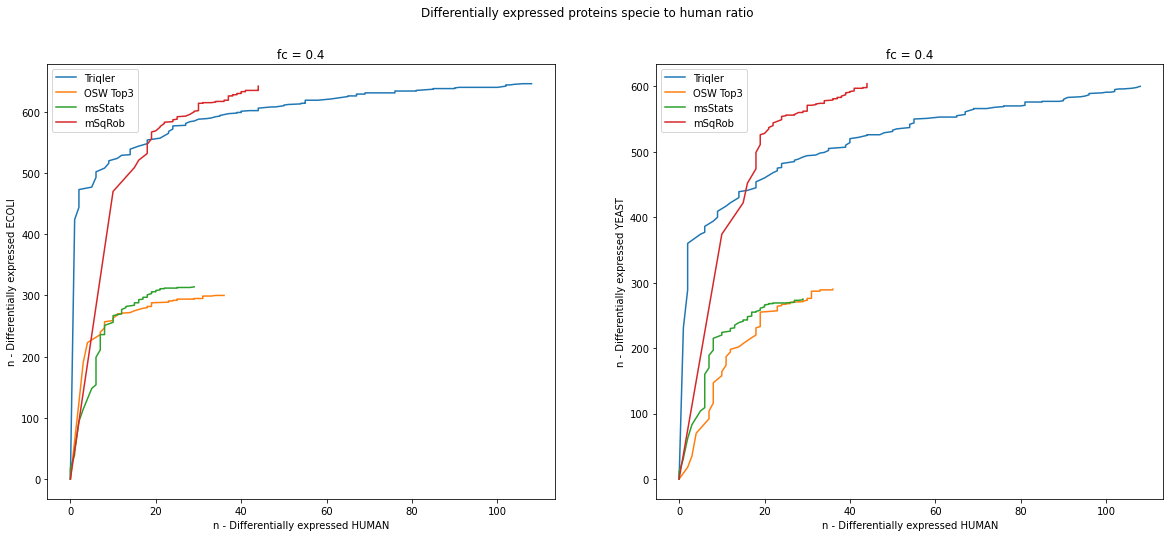
\includegraphics[width=0.3\linewidth]{../../result/report_plots/de_human_vs_de_specie.png} & 
        %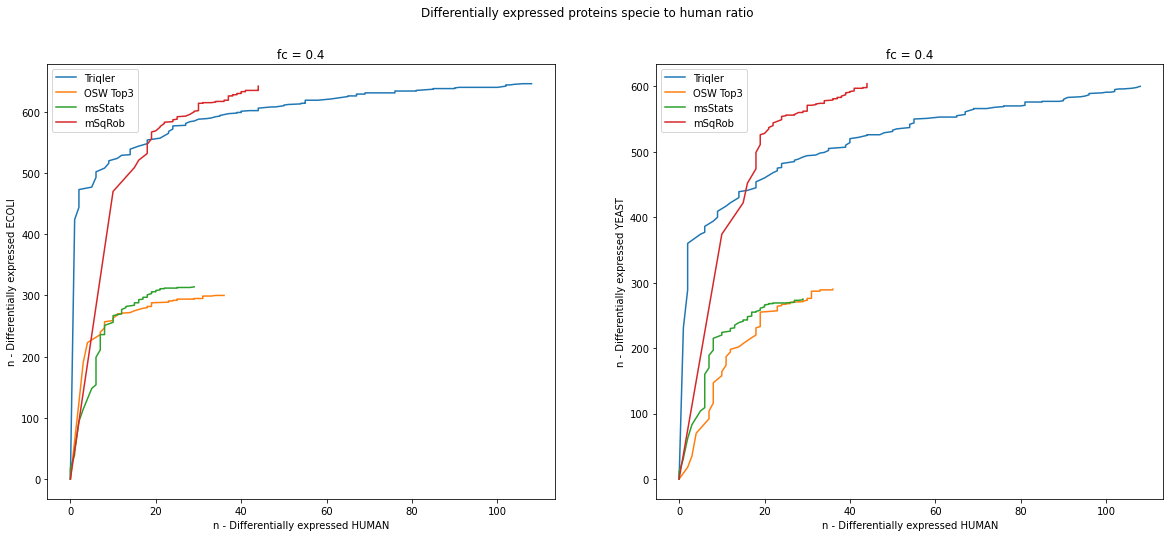
\includegraphics[width=0.3\linewidth]{../../result/report_plots/de_human_vs_de_specie.png} \\ 
        %A & B
        A 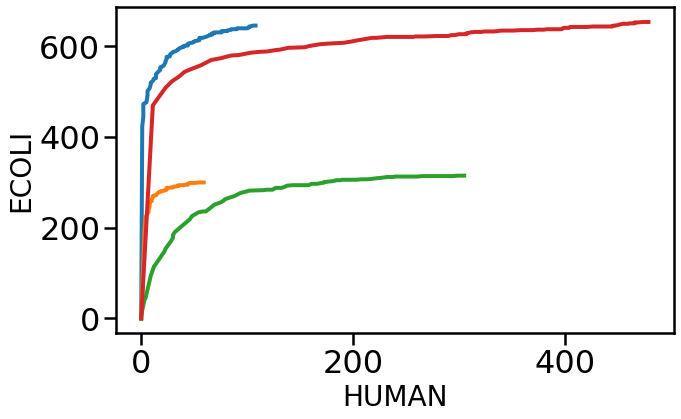
\includegraphics[width=0.5\linewidth]{../../result/report_plots/osw_de_human_vs_ecoli.png} & &%\includegraphics[width=0.3\linewidth]{} & 
        C 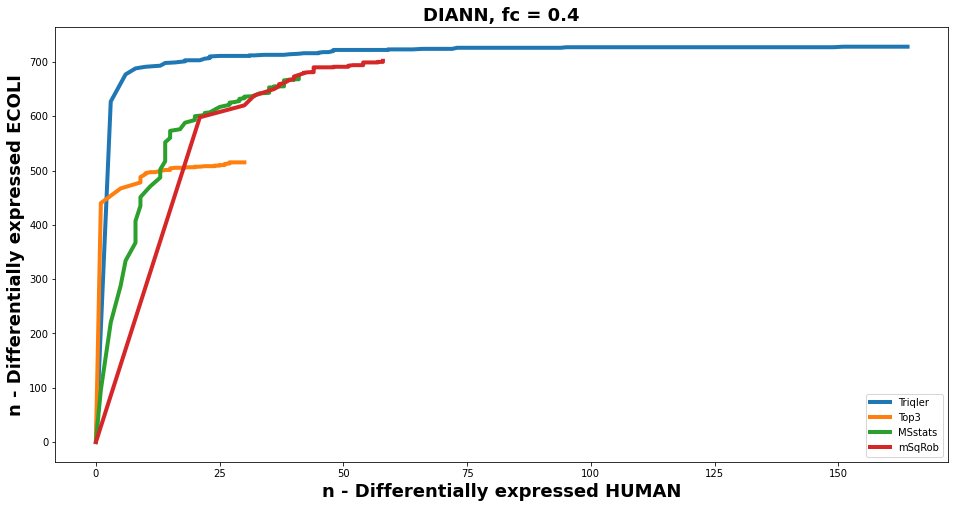
\includegraphics[width=0.5\linewidth]{../../result/report_plots/diann_de_human_vs_ecoli.png} & \\%\includegraphics[width=0.3\linewidth]{} \\ 
        B 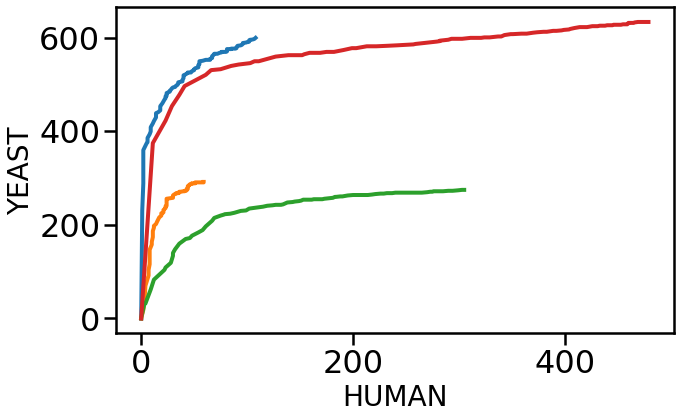
\includegraphics[width=0.5\linewidth]{../../result/report_plots/osw_de_human_vs_yeast.png} & &%\includegraphics[width=0.3\linewidth]{} & 
        D 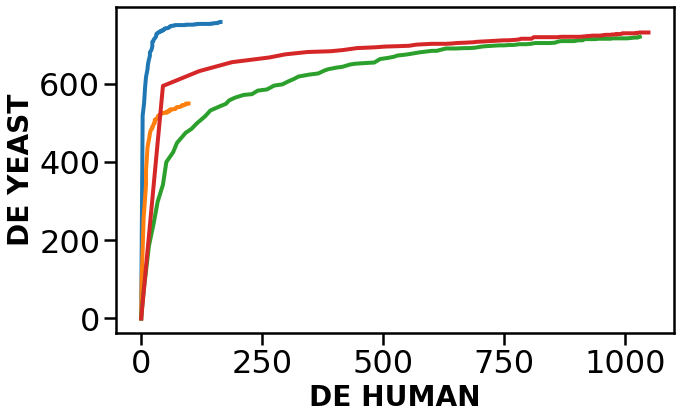
\includegraphics[width=0.5\linewidth]{../../result/report_plots/diann_de_human_vs_yeast.png} & \\%\includegraphics[width=0.3\linewidth]{} \\ 
    \end{tabular}
    \todo[inline]{Use one plot per png-file. In ech pane plot the sum of the ecoli and yeast proteins as a function of human proteins. One plot for spectral libraries, one for dia umpire.}
    \caption{{\bf Comparison of ability to differentiate differentially abundant proteins} We plotted the number of reported differentially abundant  {\em E. Coli} and Yeast proteins as a function of number of proteins from the HeLa background when sorting according to significance for (A-B) DDA generated spectral libraries and (C-D) DIA-Umpire geneated Pseudo spectra. For the test we selected a fold-change treshold of 0.4 for Triqler. \label{fig:diff_vs_hela}}
\end{figure}

\subsubsection*{Comparison of statistical calibration}

We subsequently set out to test the statistical calibration of the different summarization methods. We hence investigated the relation between the fraction of wrongly reported differential abundant proteins (i.e. the number of human proteins), and the estimated false discovery rate (See Figure \ref{fig:frac_hela_vs_fdr})
\begin{figure}[hbt]
    \centering
    \centering
    \begin{tabular}{lclc} 
        %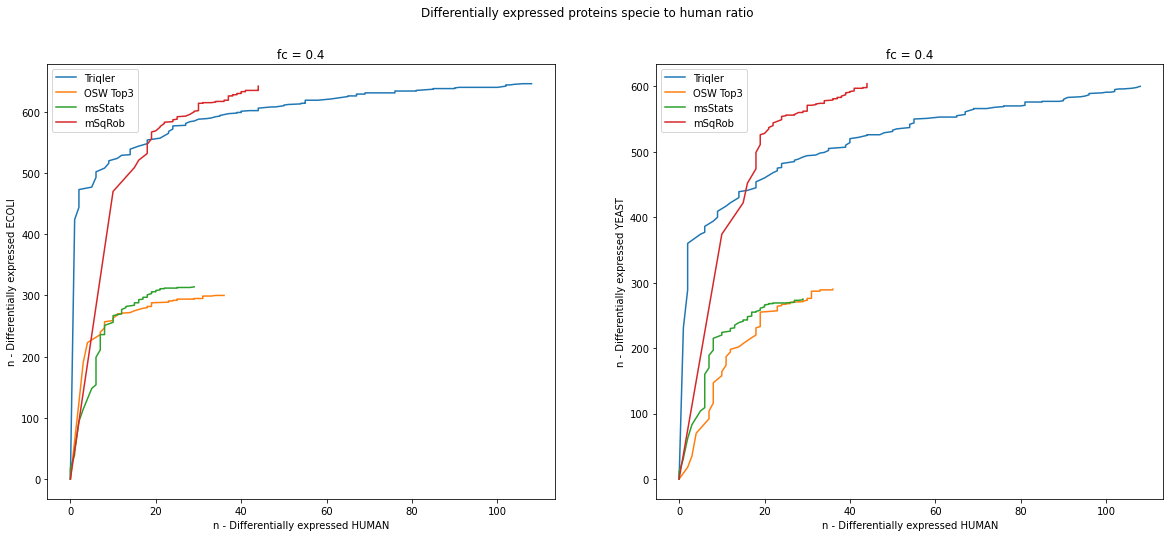
\includegraphics[width=0.3\linewidth]{../../result/report_plots/de_human_vs_de_specie.png} & 
        %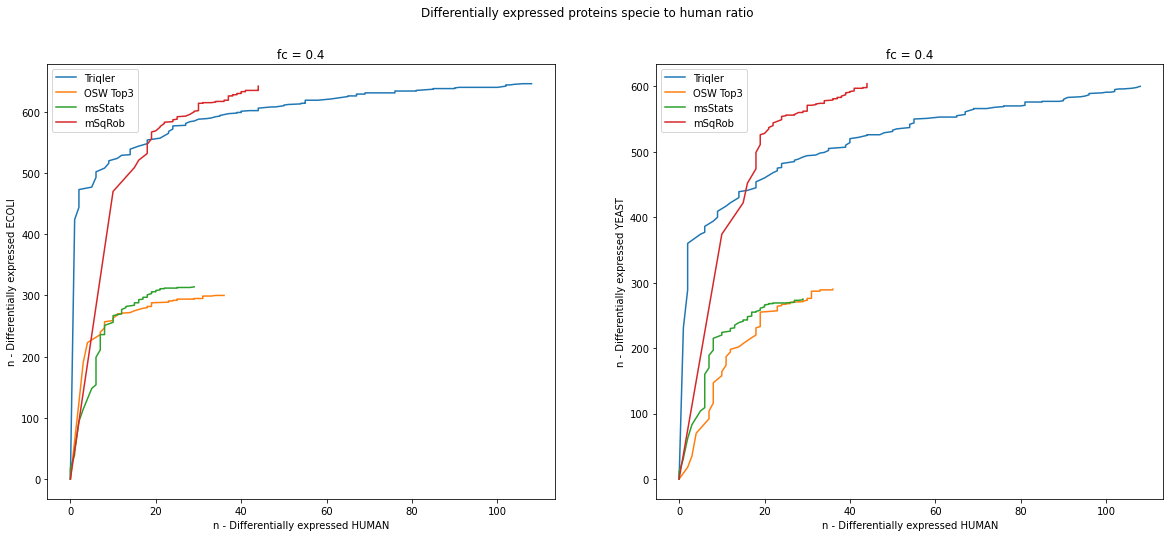
\includegraphics[width=0.3\linewidth]{../../result/report_plots/de_human_vs_de_specie.png} \\ 
        %A & B
        A 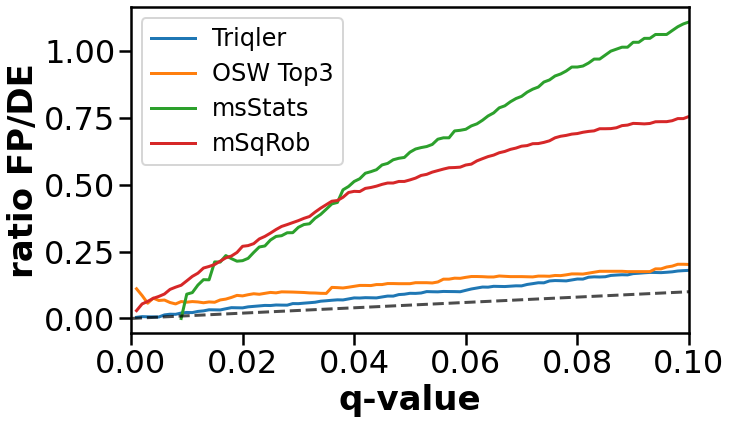
\includegraphics[width=0.5\linewidth]{../../result/report_plots/osw_FP_DE_yeast.png} & &%\includegraphics[width=0.3\linewidth]{} & 
        D 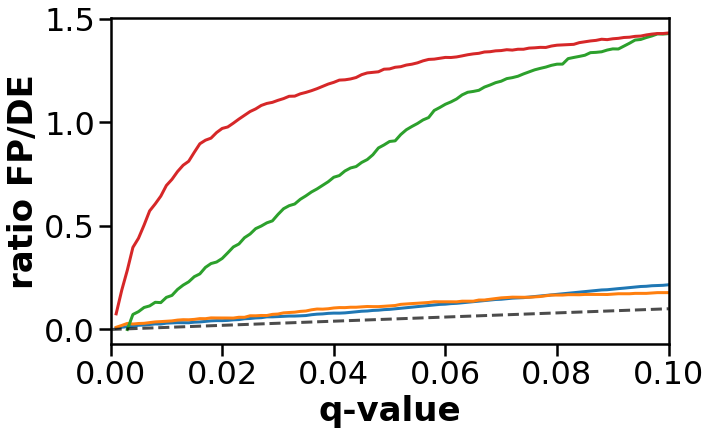
\includegraphics[width=0.5\linewidth]{../../result/report_plots/diann_FP_DE_yeast.png} & \\%\includegraphics[width=0.3\linewidth]{} \\ 
        B 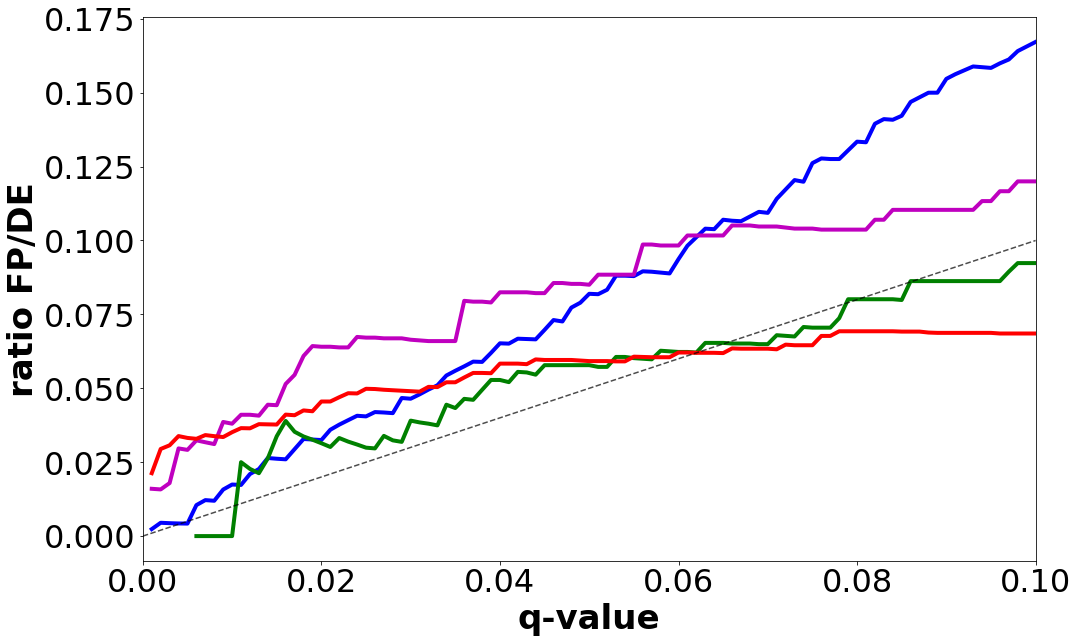
\includegraphics[width=0.5\linewidth]{../../result/report_plots/osw_FP_DE_ecoli.png} & &%\includegraphics[width=0.3\linewidth]{} & 
        E 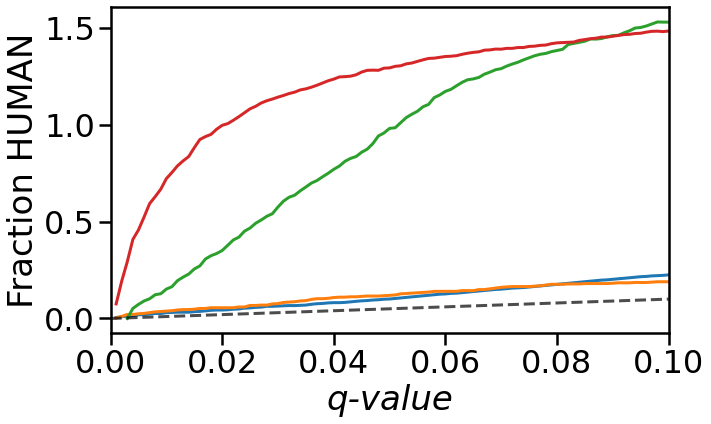
\includegraphics[width=0.5\linewidth]{../../result/report_plots/diann_FP_DE_ecoli.png} & \\%\includegraphics[width=0.3\linewidth]{} \\ 
        C 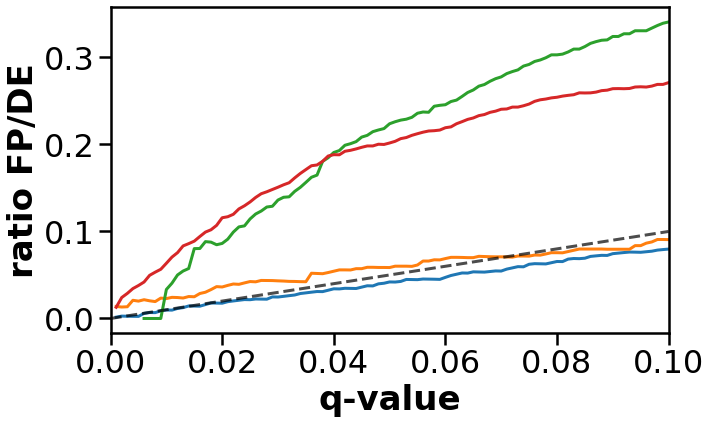
\includegraphics[width=0.5\linewidth]{../../result/report_plots/osw_FP_DE_all.png} & &%\includegraphics[width=0.3\linewidth]{} & 
        F 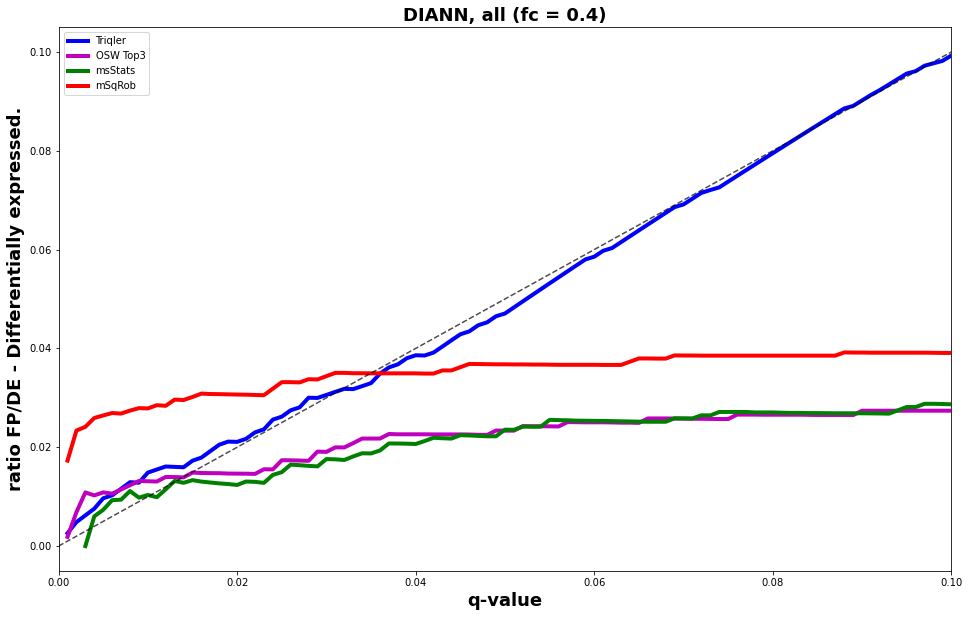
\includegraphics[width=0.5\linewidth]{../../result/report_plots/diann_FP_DE_all.png} & \\%\includegraphics[width=0.3\linewidth]{} \\ 
    \end{tabular}
    \caption{{\bf Comparison of calibration of the compared summarization methods.} We plotted the fraction of reported differentially abundant HeLa proteins as a function of $q$~value treshhold for (A-C) DDA generated spectral libraries and (D-F) DIA-Umpire geneated Pseudo spectra. \label{fig:frac_hela_vs_fdr}}
    \todo[inline]{Just plot the fraction reported human proteins to all reported proteins.(Right now I think I am not convinced we need the compensational factor -- at least not if you can not come up with an argument of why it should be there.) Use one png per subplot, and just use 2 subplots.}
\end{figure}


\subsubsection*{Constant variance}

\begin{figure}[hbt]
    \centering
    \centering
    \begin{tabular}{lclc} 
        %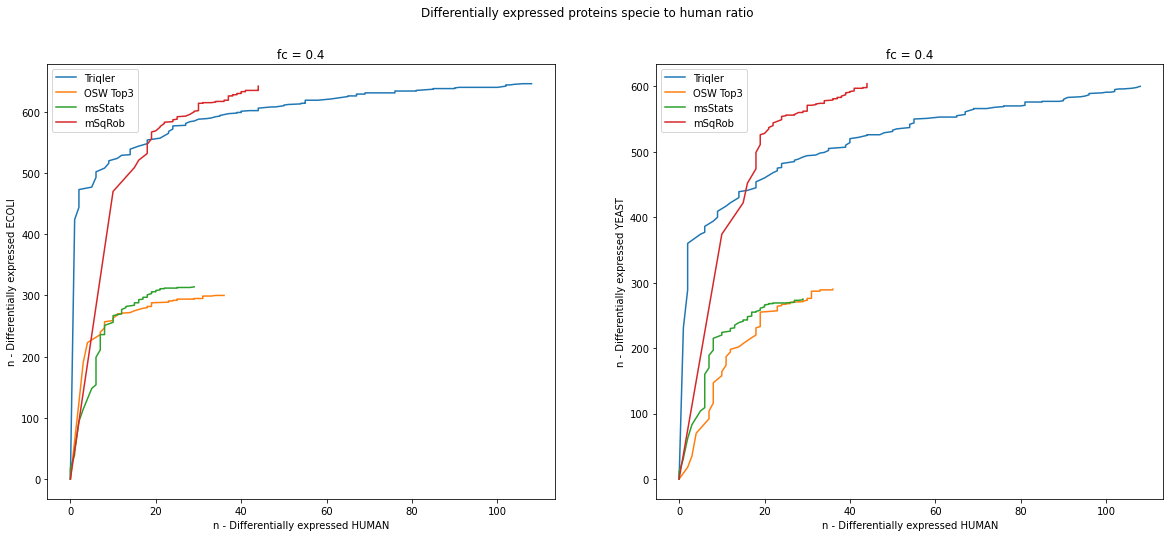
\includegraphics[width=0.3\linewidth]{../../result/report_plots/de_human_vs_de_specie.png} & 
        %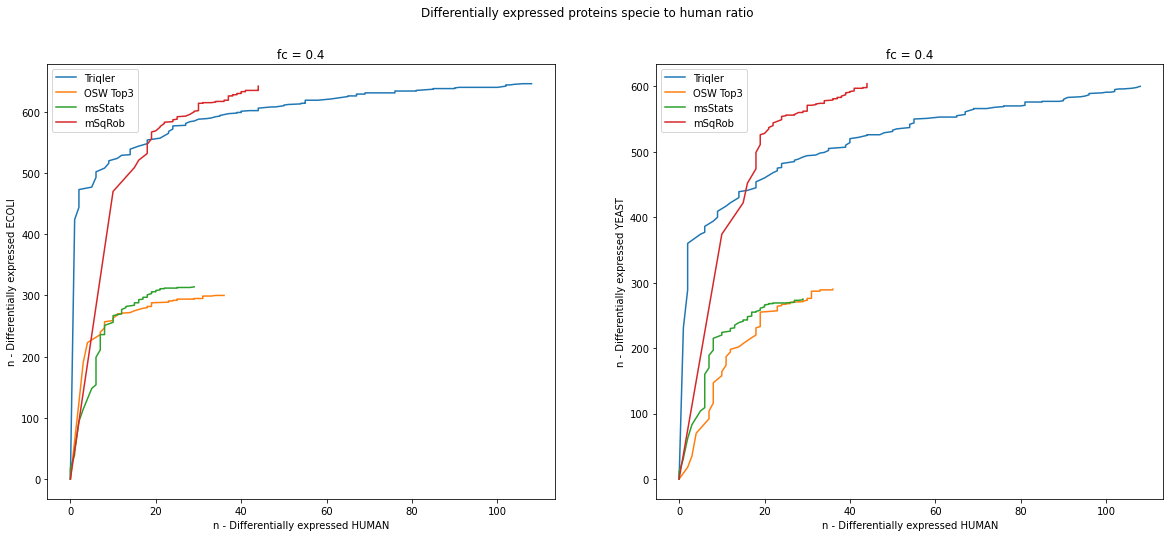
\includegraphics[width=0.3\linewidth]{../../result/report_plots/de_human_vs_de_specie.png} \\ 
        %A & B
         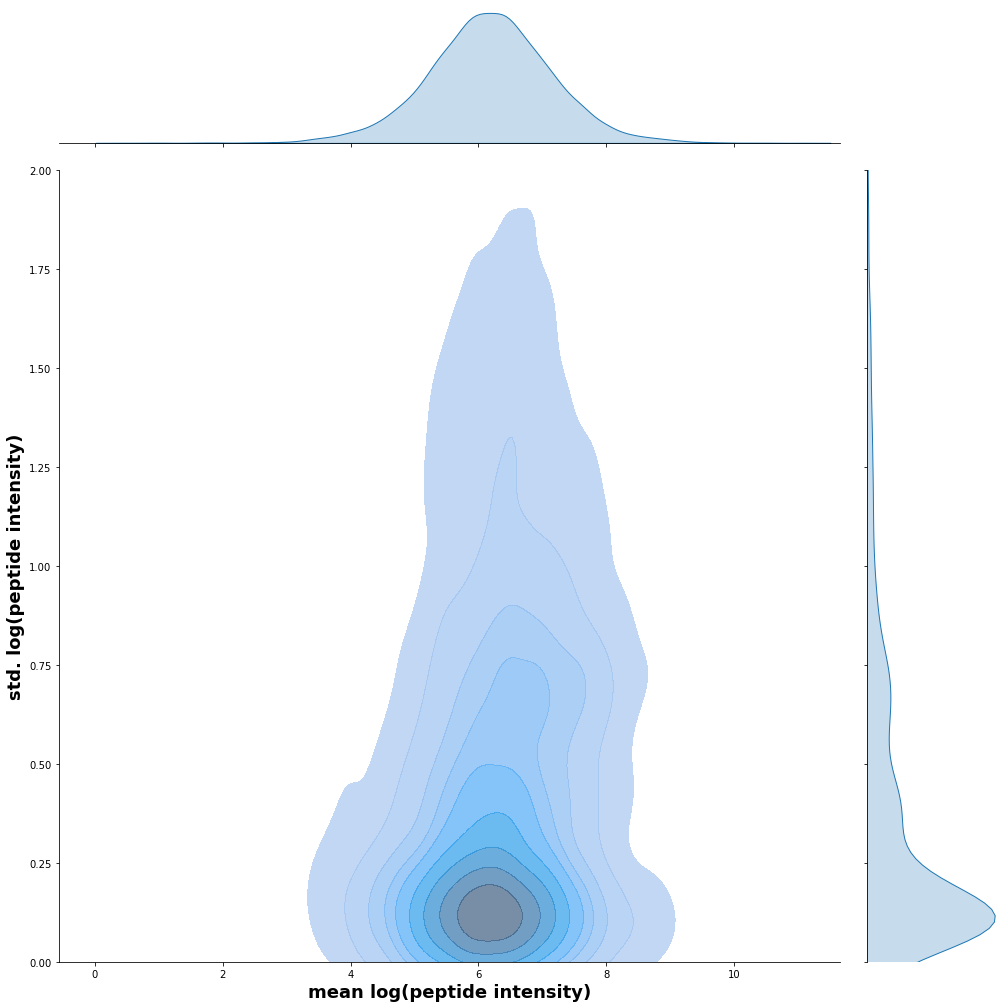
\includegraphics[width=0.5\linewidth]{../../result/report_plots/peptide_mu_vs_std.png} & &%\includegraphics[width=0.3\linewidth]{} & 

    \end{tabular}
    %\caption{{\bf mean of log2-peptide intensities against std. of log2-peptide intensities.} We plotted the mean of log2-peptide intensities against std. of log2-peptide intensities to show that the variance does not increase with the mean. The peptides where tresholded at a m_score less than 0.001. \label{fig:mu_vs_std}}
    \caption{{\bf Mean of log2-peptide intensities against std. of log2-peptide intensities.} We plotted the mean of log2-peptide intensities against std. of log2-peptide intensities to show that the variance does not increase with the mean. \label{fig:test}}
    \todo[inline]{Check if there is a log of missing values among peptides to see if they skew the std. in y-axis.}
\end{figure}

\begin{figure}[hbt]
    \centering
    %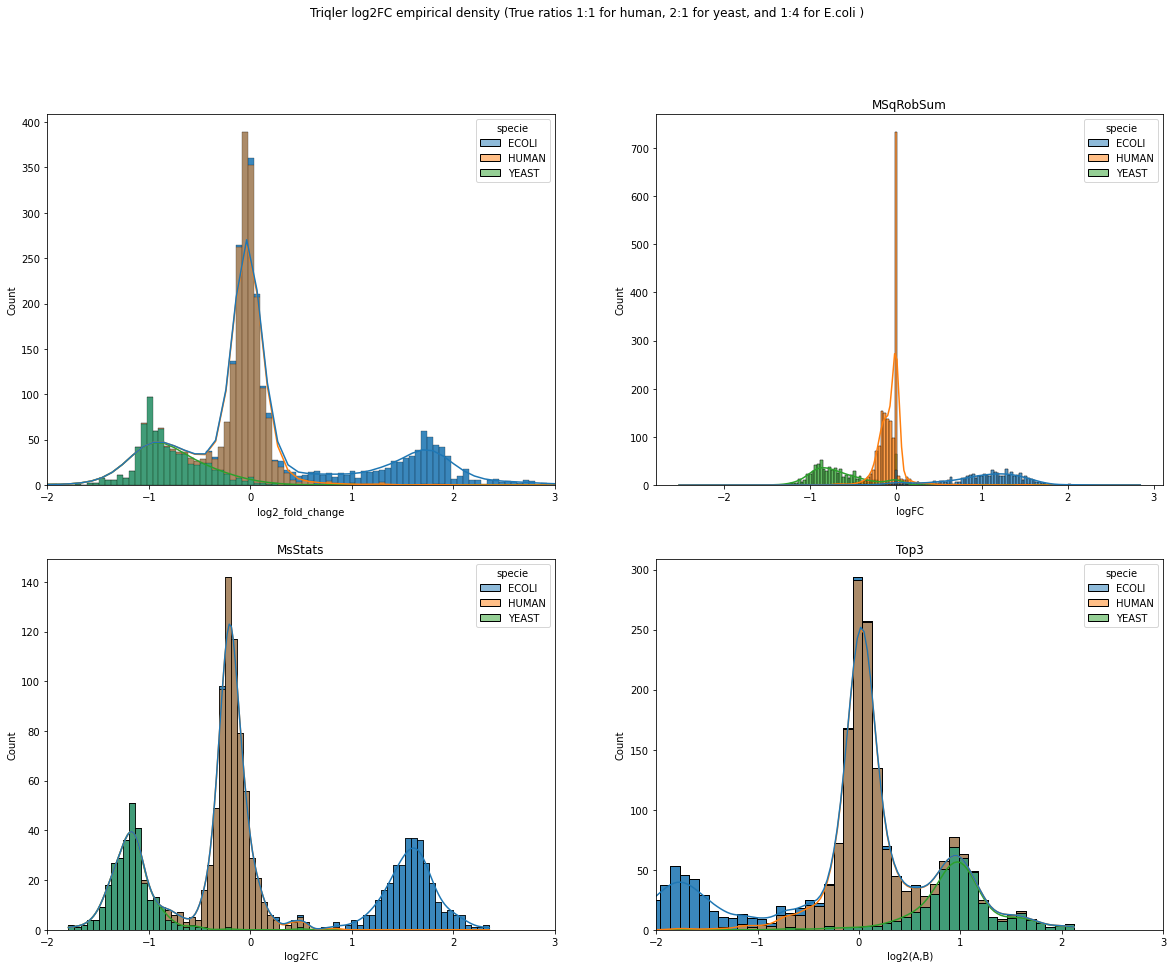
\includegraphics[width=16cm]{../../result/2021-08-13_docs_plots/intensity_plot.png}
    \begin{tabular}{lclc} 
        A  & &%\includegraphics[width=0.3\linewidth]{} & 
        E 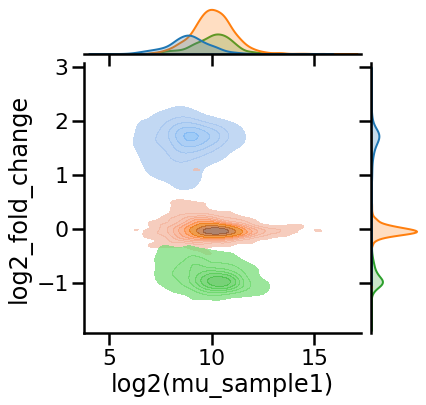
\includegraphics[width=0.3\linewidth]{../../result/report_plots/diann_scatter_triqler.png} & \\%\includegraphics[width=0.3\linewidth]{} \\ 
        B  & &%\includegraphics[width=0.3\linewidth]{} & 
        F 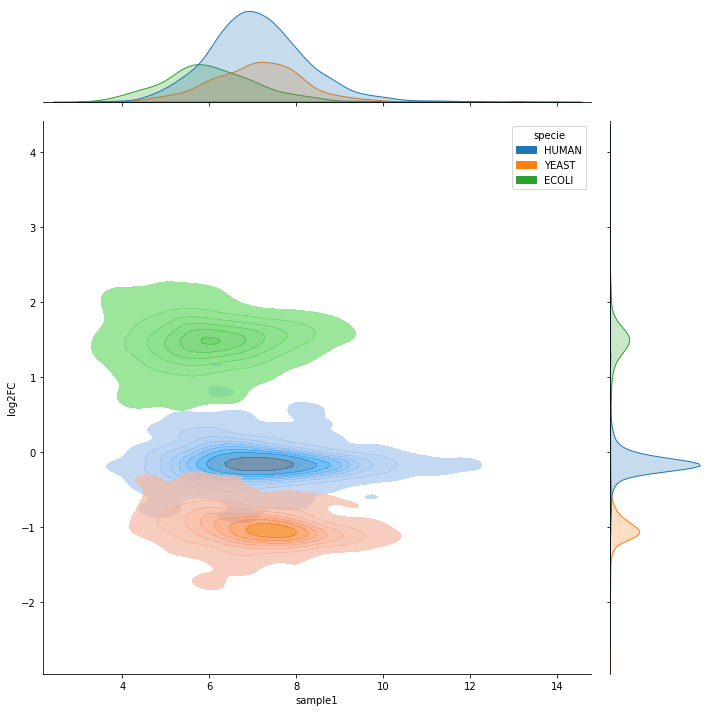
\includegraphics[width=0.3\linewidth]{../../result/report_plots/diann_scatter_msqrobsum.png} & \\%\includegraphics[width=0.3\linewidth]{} \\ 
        C  & &%\includegraphics[width=0.3\linewidth]{} & 
        G 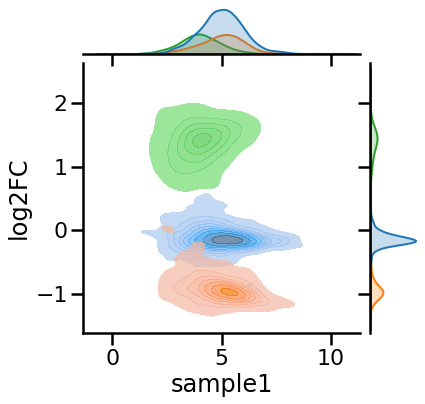
\includegraphics[width=0.3\linewidth]{../../result/report_plots/diann_scatter_msstats.png} & \\%\includegraphics[width=0.3\linewidth]{} \\ 
        D  & &%\includegraphics[width=0.3\linewidth]{} & 
        H 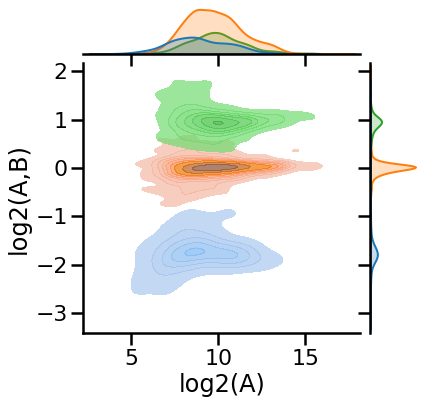
\includegraphics[width=0.3\linewidth]{../../result/report_plots/diann_scatter_top3.png} & %\includegraphics[width=0.3\linewidth]{} 
    \end{tabular}
    \todo[inline]{Make scatter for OSW as well, and how to do with fig sizing?.}
    \caption{{\bf Comparison of reported fold change distributions.} We used peptide data from (A-D) DDA spectrum libraries and (E-H) psedo spectra as generated by 
    (A,E) Triqler, (B,F) MSqRobSum, (C,G) MSstats, and (D,H) Top-3. \label{fig:fc_histogram}}
\end{figure}



\todo{Finish the truncated distribution fitting}

\begin{comment}
\subsection*{Protein quantification}

Log-transformed ratios (log2(A//B)) of proteins (humans proteins in orange, yeast proteins in green, and E. Coli proteins in blue) were plotted for each benchmarked software over the log-transformed intensity of sample A. The dashed horizontal line represents the expected log-fold change, while the fitted dashed line represents a linear regression for each species. Fig. \ref{fig:OSW_scatter} shows the results for OpenSwath and fig. \ref{fig:OSW_scatter} shows the results for DIA-NN. TOP3 and MsStat gives least biased results as protein intensities gets higher. Triqler gives the most biased results. 

\begin{figure}[H]
    \centering
    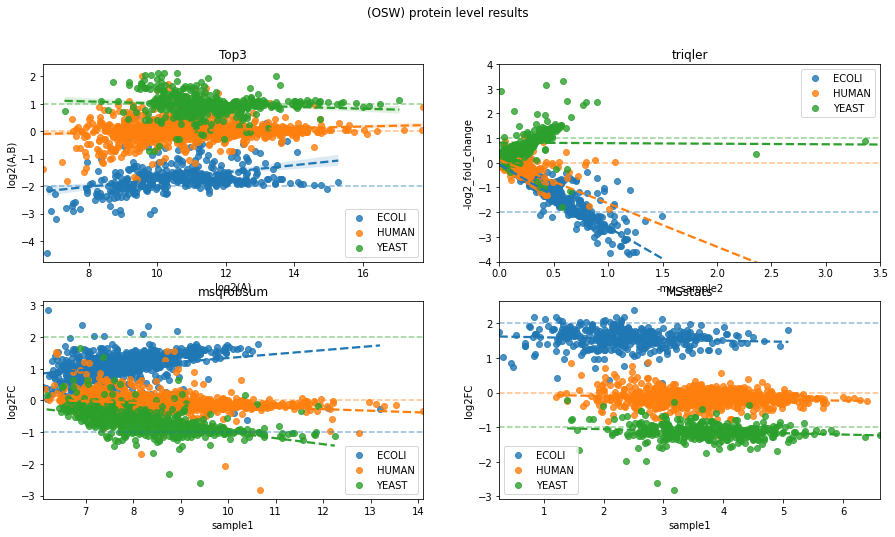
\includegraphics[width=16cm]{../../result/2021-08-13_docs_plots/OSW_protein_level_benchmark_scatter.png}
    \caption{OSW Protein level results from Triqler, Top3, MSstats and MSqRobSum.}
    \label{fig:OSW_scatter}
\end{figure}

\begin{figure}[H]
    \centering
    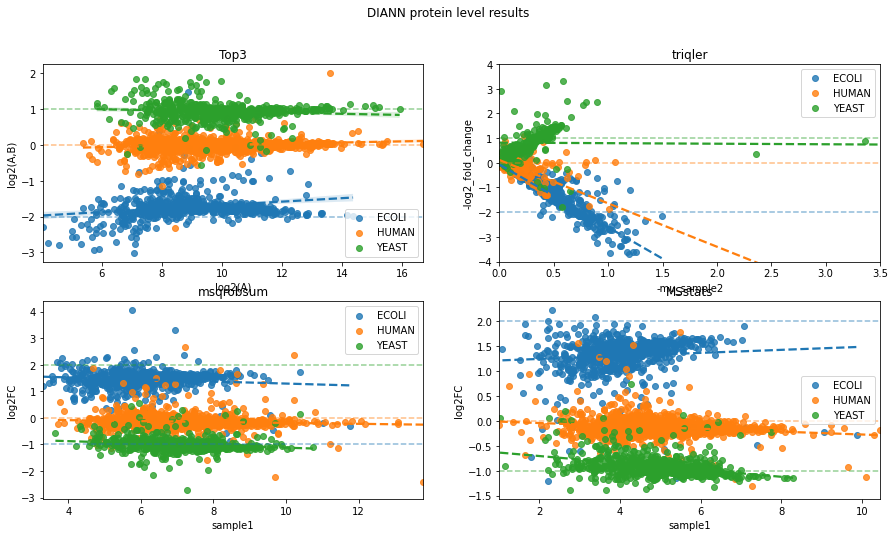
\includegraphics[width=16cm]{../../result/2021-08-13_docs_plots/DIANN_protein_level_benchmark_scatter.png}
    \caption{DIANN Protein level results from Triqler, Top3, MSstats and MSqRobSum.}
    \label{fig:OSW_scatter}
\end{figure}

Fig. \ref{fig:intensity_distribution} and \ref{fig:DIANN_intensity_distribution} show the protein quantity distributions with the different species; human (orange), E. Coli (blue), and yeast (green) highlighted in different colors for OSW \ref{fig:intensity_distribution} and DIA-NN \ref{fig:DIANN_intensity_distribution}. The human and yeast distribution apex is not centered at 0 in MsStats and MSqRob, while it is centered for triqler and top3. Likewise, the distribution for e.coli is closer to the true log2 fold change ratios for triqler and top3, while the apexes are skewed towards 0 for MsStats and MSqRob for both OSW and DIA-NN.     

\begin{figure}[H]
    \centering
    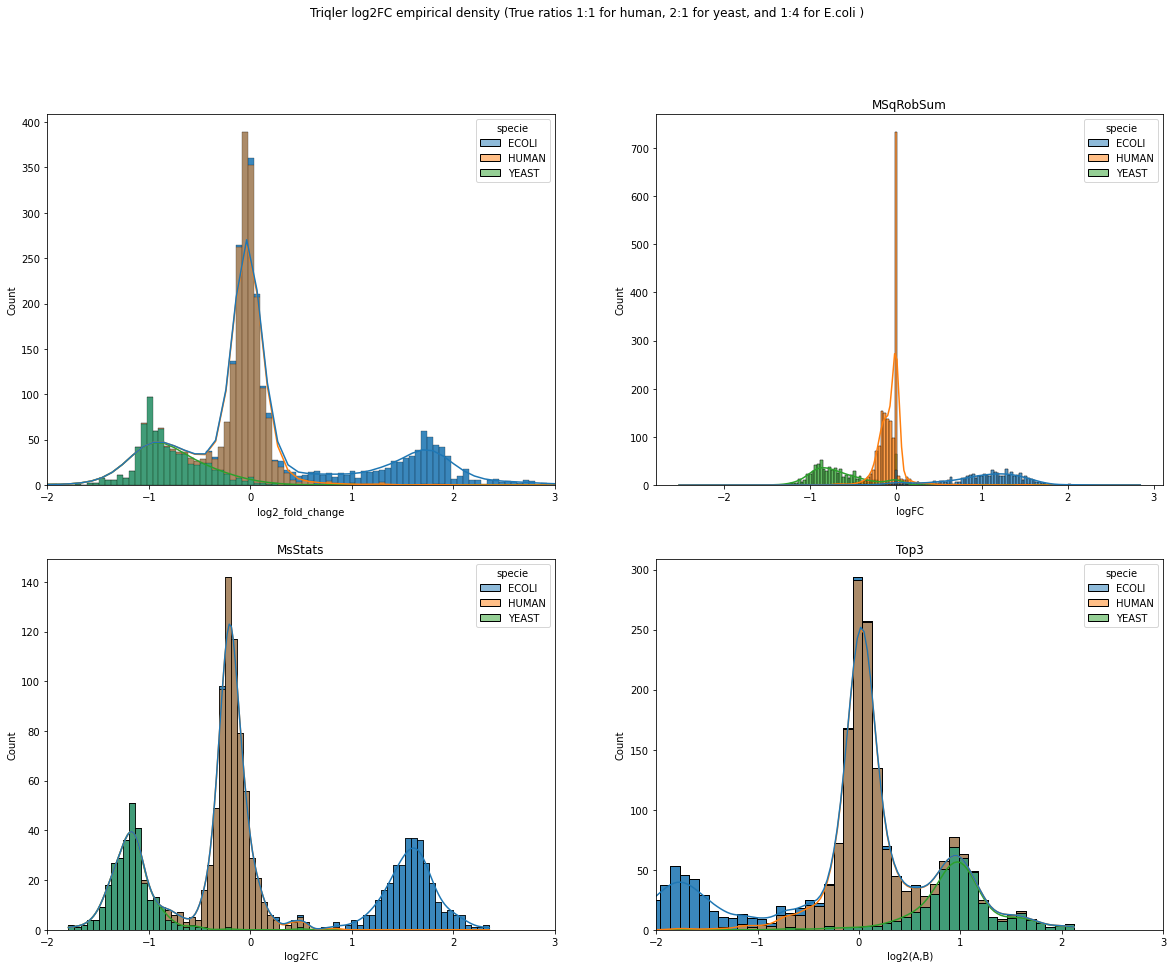
\includegraphics[width=16cm]{../../result/2021-08-13_docs_plots/intensity_plot.png}
    \caption{OSW Protein quantity distributions from Triqler, Top3, MSstats and MSqRobSum.}
    \label{fig:intensity_distribution}
\end{figure}

\begin{figure}[H]
    \centering
    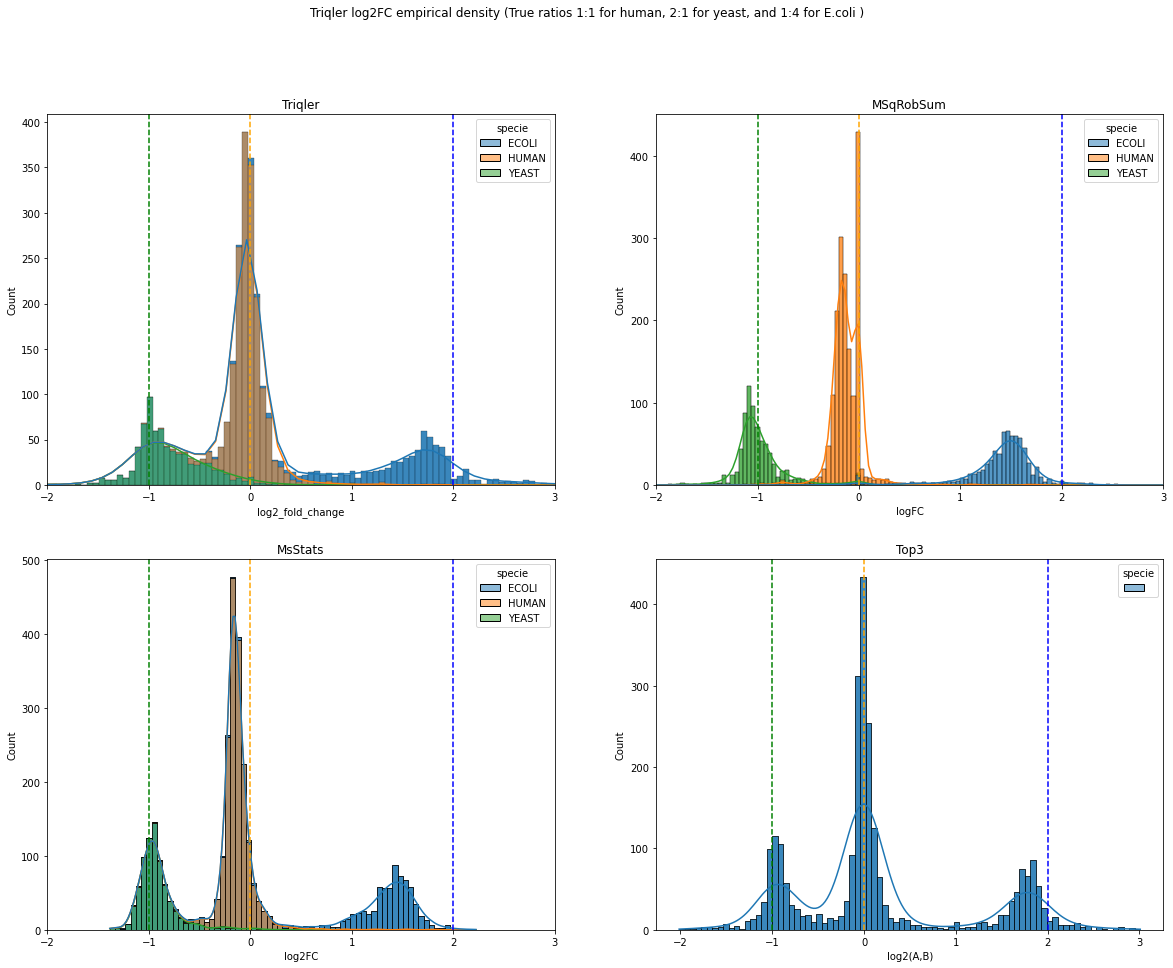
\includegraphics[width=16cm]{../../result/2021-08-13_docs_plots/DIANN_intensity_plot.png}
    \caption{DIANN Protein quantity distributions from Triqler, Top3, MSstats and MSqRobSum.}
    \label{fig:DIANN_intensity_distribution}
\end{figure}


Fig. \ref{fig:osw_n_diff_exp} and \ref{fig:DIANN_n_diff_exp} shows that the number of differentially abundance proteins is significantly higher for Triqler and MSqRobSum at different false discovery rates. MSqRobSum has a slightly higher number of differentially abundant proteins than triqler for OSW, and Triqler has slightly higher number of differentially abundant proteins for DIA-NN. The difference between the number of differentially abundant proteins are also smaller for MsStats and triqler and MSqRobSum for DIA-NN. 

\begin{figure}[H]
    \centering
    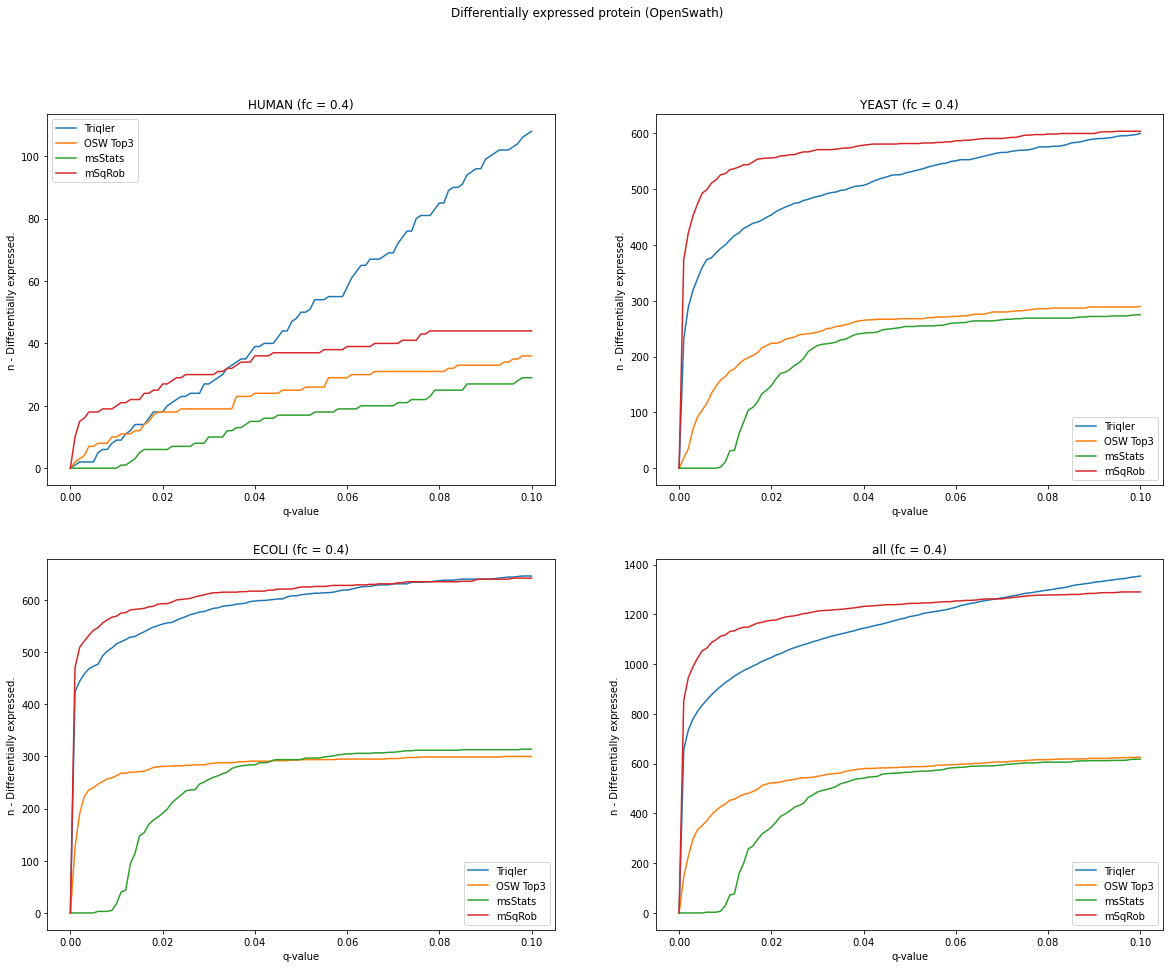
\includegraphics[width=16cm]{../../result/2021-08-13_docs_plots/n_diff_expressed.png}
    \caption{OSW Number of differentially abundant proteins for an OpenSwath analysis with triqler, top3, MsStats and MSqRobSum protein summarization.}
    \label{fig:osw_n_diff_exp}
\end{figure}

\begin{figure}[H]
    \centering
    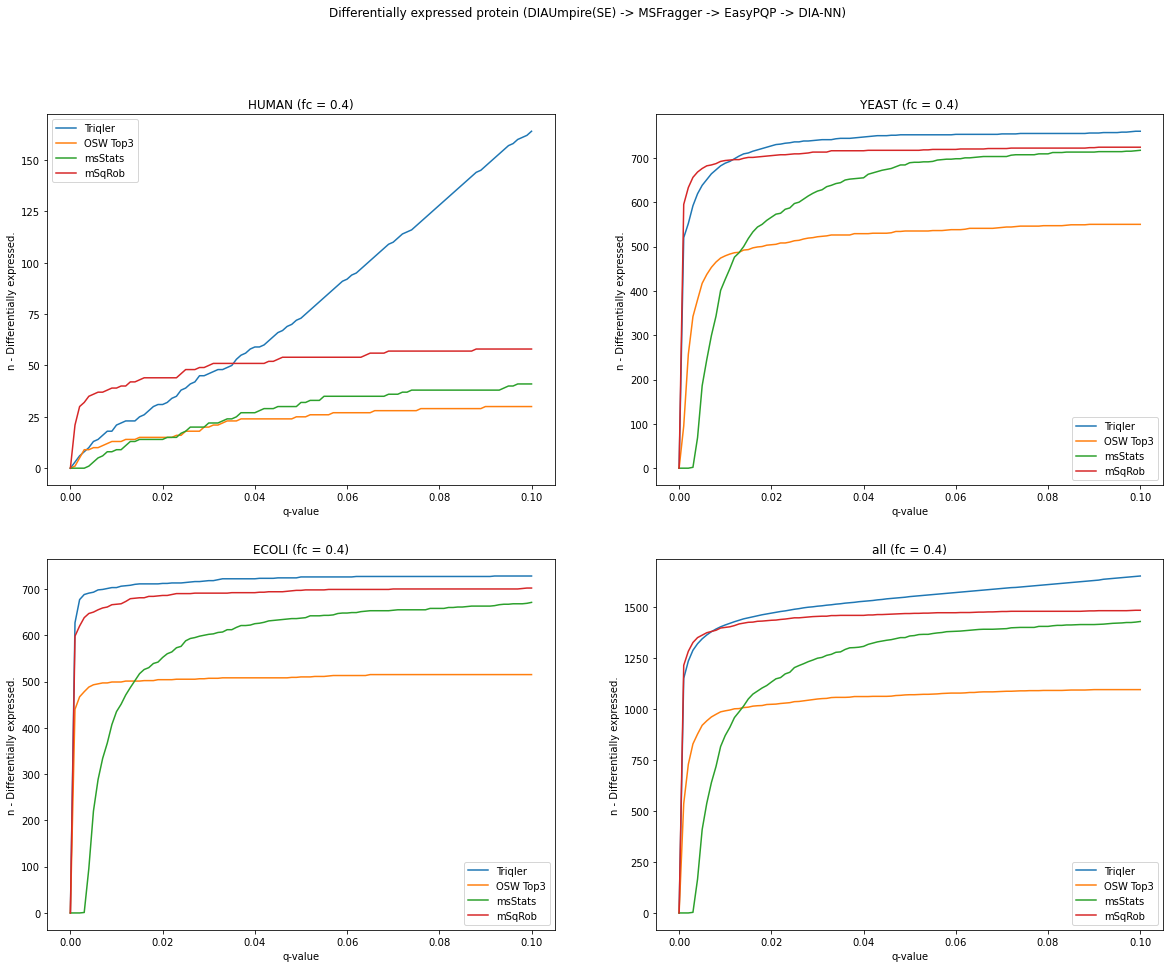
\includegraphics[width=16cm]{../../result/2021-08-13_docs_plots/DIANN_n_diff_expressed.png}
    \caption{DIANN Number of differentially abundant proteins for an OpenSwath analysis with triqler, top3, MsStats and MSqRobSum protein summarization.}
    \label{fig:DIANN_n_diff_exp}
\end{figure}



Fig. \ref{fig:osw_n_diff_exp} and \ref{fig:DIANN_n_diff_exp} shows that the ratio of false positives (human proteins) to the number of differentially abundant proteins for a given q-value level is more linear for triqler. At log2FC = 2 all methods are conservative at low q-values and anti-conservative at higher q-values. Triqler is better calibrated for low q-values and gets more conservative as the q-value threshold is increased. Top3, MsStats, and MSqRob are more conservative at low q-values and get less conservative as the q-value threshold increases.  

   
\begin{figure}[H]
    \centering
    \includegraphics[width=16cm]{../../result/2021-08-13_docs_plots/calibration_plot_scaled.png}
    \caption{OSW Q-value (x-axis) and false positive / number differentially abundant protein (y-axis) ratio.}
    \label{fig:osw_n_diff_exp}
\end{figure}

\begin{figure}[H]
    \centering
    \includegraphics[width=16cm]{../../result/2021-08-13_docs_plots/DIANN_calibration_plot.png}
    \caption{DIANN Q-value (x-axis) and false positive / number differentially abundant protein (y-axis) ratio.}
    \label{fig:DIANN_n_diff_exp}
\end{figure}

Fig. \ref{fig:osw_de_human_vs_de_specie} and \ref{fig:DIANN_de_human_vs_de_specie} shows  

\begin{figure}[H]
    \centering
    \includegraphics[width=12cm]{../../result/2021-08-13_docs_plots/de_human_vs_de_specie.png}
    \caption{OSW Number of differentially abundant humans (x-axis) and differentially abundant e.coli and yeast (y-axis).}
    \label{fig:osw_de_human_vs_de_specie}
\end{figure}

\begin{figure}[H]
    \centering
    \includegraphics[width=12cm]{../../result/2021-08-13_docs_plots/DIANN_de_human_vs_de_specie.png}
    \caption{DIANN Number of differentially abundant humans (x-axis) and differentially abundant e.coli and yeast (y-axis).}
    \label{fig:DIANN_de_human_vs_de_specie}
\end{figure}

\end{comment}

\section*{Discussion}

Here we have shown that Triqler operates well for DIA data, despite originally intended for DDA data. We also find that Triqler outperforms other protein summarization methods on our engineered benchmark set, both in terms of sensitivity and accuracy in its error estimates.

We do see some differences in how DIA and DDA ppetide-level abundance data appear. For instance there are more missing values in DDA than DIA data. Howwever, we find that qualatively the types of data are similar, at leas tin the sense that Triqler's underlying assumption of missing values seem to be as valid for DDA and DIA data.


\section*{Acknowledgements}


\section*{Funding}

This work was supported by grants from the Swedish Research Council (grant 2017-04030) 

\section*{Supporting information}

\bibliographystyle{plain}
%\bibliography{benchmark}
\bibliography{benchmark.bib}
\end{document}



